\documentclass[11pt,a4paper,english,greek,twoside]{thesis_master}

\usepackage[utf8]{inputenc}
\usepackage{graphicx}
\usepackage{epstopdf}
\usepackage{indentfirst}
\usepackage{verbatim}
\usepackage{amsmath}
\usepackage{empheq}
\usepackage{array}
\usepackage{amsthm}
\usepackage{amssymb}
\usepackage{amsfonts}
\usepackage{latexsym}
\usepackage{float}
\bibliographystyle{hellas}
\usepackage{hyphenat}
\usepackage{makeidx}
\usepackage{csquotes}
\usepackage{wrapfig}
\usepackage{lipsum}
\usepackage{mathtools}
\usepackage{commath}
\usepackage{xcolor}
\usepackage{listings}
\usepackage{subfigure}
\usepackage{color, soul}
\usepackage{multirow}
\usepackage{array}
\usepackage{booktabs}
\usepackage{fixltx2e}
\usepackage{xr}
\usepackage[framed,numbered,autolinebreaks,useliterate]{mcode}
\addto\captionsgreek{%
  \renewcommand{\indexname}{Ευρετήριο όρων}%
}
\makeindex

% 1.5 spacing
\renewcommand{\baselinestretch}{1.2}

% latin text (and greek text)
\newcommand{\tl}[1]{\textlatin{#1}}
\newcommand{\tg}[1]{\textgreek{#1}}

% typeset short english phrases
\newcommand{\en}[1]{\foreignlanguage{english}{#1}}

% typeset source code
\newcommand{\src}[1]{{\tt\en{#1}}}

% typeset a backslash
\newcommand{\bkslash}{\en{\symbol{92}}}

\newtheorem{definition}{Ορισμός}
\newtheorem{proposition}{Πρόταση}
\newtheorem{theorem}{Θεώρημα}
\newtheorem{corollary}{Συμπέρασμα}
\newtheorem{lemma}{Λήμμα}
\newtheorem{example}{Παράδειγμα}
\newtheorem{remark}{Σημείωση}
\newtheorem{notation}{Συμβολισμός}
\newtheorem{law}{Νόμος}
\renewcommand{\thedefinition}{\arabic{chapter}.\arabic{definition}}
\renewcommand{\theproposition}{\arabic{chapter}.\arabic{proposition}}
\renewcommand{\thetheorem}{\arabic{chapter}.\arabic{theorem}}
\renewcommand{\thecorollary}{\arabic{chapter}.\arabic{corollary}}
\renewcommand{\thelemma}{\arabic{chapter}.\arabic{lemma}}
\renewcommand{\theexample}{\arabic{chapter}.\arabic{example}}
% \newcommand{\set}[1]{\left\{#1\right\}}
\newcommand{\To}{\Longrightarrow}
\newcommand{\xml}{\en{XML}}

\selectlanguage{greek}

\hyphenation{ο-ποί-α}

%%%%%%%%%%%%%%%%%%%%%%%%%%%%%%%%%%%%%%%%%%%%%%%%%%%%%
%% THESIS INFO 
%%
%
% Τίτλος Πτυχιακής Εργασίας
	\title{Προγραμματισμός κώδικα επανάληψης-συσσώρευσης (\en{repeat-accumulate}) και προσομοίωσή του σε περιβάλλον \en{AWGN}}
% "του" ή "της", ανάλογα με το φύλο του σπουδαστή
	\edef\toutis{του}
% Ονοματεπώνυμο σπουδαστή (ΚΕΦΑΛΑΙΑ, γενική πτώση)
	\edef\authorNameCapital{ΠΑΝΟΥΡΓΙΑ Δ. ΧΡΗΣΤΟΥ}
% Ονοματεπώνυμο σπουδαστή (πεζά, ονομαστική πτώση)
	\author{Χρήστος Δ. Πανουργιάς}
% Ονοματεπώνυμο Επιβλέποντα Καθηγητή
	\supervisor{Χρήστος E. Δημάκης}
% Τίτλος Επιβλέποντα Καθηγητή
	\edef\supervisorTitle{Επίκουρος Καθηγητής}
% "Επιβλέπων" ή "Επιβλέπουσα", ανάλογα με το φύλο του Επιβλέποντα Καθηγητή
	\edef\supervisorMaleFemale{Επιβλέπων}
% Τόπος, μήνας και έτος
	\edef\thesisPlaceDate{Θεσσαλονίκη, Φεβρουάριος 2018}
%%%%%%%%%%%%%%%%%%%%%%%%%%%%%%%%%%%%%%%%%%%%%%%%%%%%%


\begin{document}
\selectlanguage{greek}
\maketitle

\frontmatter
% Αφιέρωση
	\thesisDedication{Στην Αγγελική}
% Ευχαριστίες
	\begin{acknowledgements}
Θα ήθελα καταρχήν να ευχαριστήσω τον Επίκουρο καθηγητή κ. Χρήστο Ε. Δημάκη, για την επίβλεψη αυτής της διπλωματικής εργασίας καθώς και για την ευκαιρία που μου έδωσε να την εκπονήσω. Επίσης ευχαριστώ ιδιαίτερα τον υποψήφιο διδάκτορα Κωνσταντή Αρκουδογιάννη για την καθοδήγησή του και την εξαιρετική συνεργασία που είχαμε καθ' όλη τη διάρκεια της εκπόνησης αυτής της εργασίας. Τέλος θα ήθελα να ευχαριστήσω τον πατέρα μου για την καθοδήγηση και την ηθική συμπαράσταση που μου προσέφερε όλα αυτά τα χρόνια.
\end{acknowledgements}

% Πίνακας Περιεχομένων
	\tableofcontents
% Περίληψη
	\begin{abstract}
Στη σύγχρονη εποχή, οι ψηφιακές τηλεπικοινωνίες αποτελούν ένα εργαλείο που αποκτά συνεχώς περισσότερες πρακτικές εφαρμογές (\en{LTE-A, Wifi, DVB-S}). Αυτό οφείλεται, σε σημαντικό βαθμό, στη χρήση τεχνικών κωδικοποίησης καναλιού. Μέσω αλγορίθμων επαναληπτικής αποκωδικοποίησης (\en{iterative decoding algorithms}), έχει καταστεί δυνατή η λειτουργία των σύγχρονων τηλεπικοινωνιακών συστημάτων κοντά στο όριο χωρητικότητας, οδηγώντας σε γρήγορη και αξιόπιστη επικοινωνία.
Λόγω αυτού, η τεχνολογική έρευα αναζητά μεθόδους παραλληλοποίησης της λειτουργίας των παραπάνω αλγορίθμων μέσω της υλοποίησής τους με σύγχρονες μονάδες επεξεργασίας γραφικών (\en{GPU}), οι οποίες προσφέρουν αρχιτεκτονικές πολλαπλών πυρήνων και υψηλής ταχύτητας μνήμη. Το αποτέλεσμα είναι η χρήση τους να γίνεται ολοένα και πιο διαδεδομένη, σε πληθώρα εφαρμογών.

Στόχος της διπλωματικής αυτής εργασίας, είναι ο προγραμματισμός ενός \en{LDPC Repeat-accumulate} κώδικα με βάση το πρότυπο \en{DVB-S2} σε \en{C++}, η καταγραφή και παρουσίαση των επιδόσεων του και η εξέταση δυνατότητας παραλληλοποίησης του, μέσω προγραμματισμού σε \en{GPU} με βάση την αρχιτεκτονική \en{CUDA}.
\end{abstract}

\begin{abstracteng}
\tl{In the modern age, digital communications consist a tool that constantly acquires more and more practical application (LTE-A, Wifi, DVB-S). This is due, to a significant extent, to the utilization of channel coding schemes. Through iterative decoding algorithms, it has been made possible for modern digital communication systems to operate close to their capacity level, leading to fast and reliable communication. Because of that, technological research is seeking ways of parallelizing these algorithms, by utilizing their development on modern graphical processing units (GPU), which offer multiple core architectures and fast memories. As a result, their use is being more and more wide, in a multitude of applications} 

\tl{This diploma thesis aims to the development of an LDPC Repeat-accumulate code, based on the DVB-S2 protocol in C++, to the recording and presentation of its performance and to examine the capability of parallelization, via its development on a GPU, using the CUDA architecture.}

\end{abstracteng}
% Κατάλογος Σχημάτων
	\listoffigures
% Κατάλογος Πινάκων
	\listoftables

%%%%%%%%%%%%%%%%%%%%%%%%%%%%%%%%%%%%%%%%%%%%%%%%%%%%%
%% INCLUDE YOUR CHAPTERS/SECTIONS HERE
%%
\mainmatter
% Κεφάλαια
 	\chapter{\selectlanguage{greek}Εισαγωγή}
Το πρωτεύον πρόβλημα της επικοινωνίας ορίζεται από τον \en{Claude E. Shannon}, στην καθοριστική εργασία του το 1948, ως η αναπαραγωγή σε ένα σημείο ενός μηνύματος που επιλέγεται σε άλλο σημείο, κατά το δυνατόν ακριβής. Ο σχεδιασμός του τηλεπικοινωνιακού συστήματος πρέπει να είναι τέτοιος, ώστε αυτό να λειτουργεί για κάθε δυνατή επιλογή μηνύματος πληροφορίας, μιας και τη στιγμή σχεδιασμού το ακριβές αυτό μήνυμα δεν είναι γνωστό \cite{shannon1948mathematical}.
\begin{figure}[h]
\center{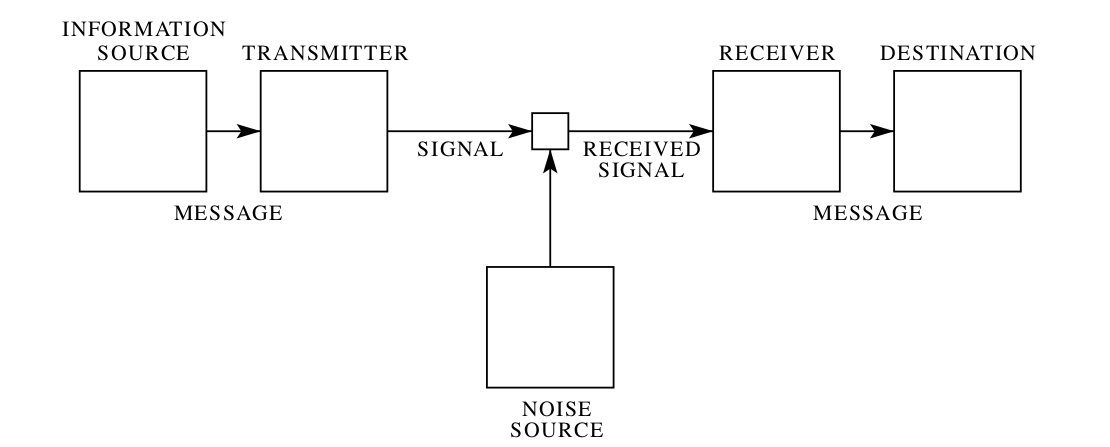
\includegraphics[width=0.75\linewidth]{figures/comm_system.png}}
\caption{Σχηματικό διάγραμμα τυπικού τηλεπικοινωνιακού συστήματος}
\label{fig:telecom system}
\end{figure}

Στο παραπάνω σχήμα (Σχήμα \ref{fig:telecom system}) φαίνεται το μπλοκ διάγραμμα ενός τυπικού τηλεπικοινωνιακού συστήματος, και τα βασικά μέρη από τα οποία αποτελείται: την πηγή πληροφορίας, τον πομπό, όπου γίνεται μετατροπή του μηνύματος πληροφορίας σε σήμα κατάλληλο για μετάδοση, το κανάλι, μέσω του οποίου γίνεται η μετάδοση, τον δέκτη, όπου γίνεται λήψη του σήματος και ανάκτηση του αρχικού μηνύματος και τέλος, τον τελικό προορισμό της πληροφορίας.

Το σχήμα \ref{fig:telecom system 2} δείχνει αναλυτικότερα τα κύρια μέρη από τα οποία αποτελείται το τηλεπικοινωνιακό σύστημα που περιγράφηκε. Tο στάδιο της κωδικοποίησης πηγής (\en{source encoding}) δεν μας απασχολεί, οπότε θεωρείται πως η πηγή εκπέμπει μια διακριτή ακολουθία από ανεξάρτητα και ομοιόμορφα κατανεμημένα (\en{independent \& identically distributed - i.i.d.}) \en{bits}.

\en{\lipsum[1]}

\begin{figure}[h]
\center{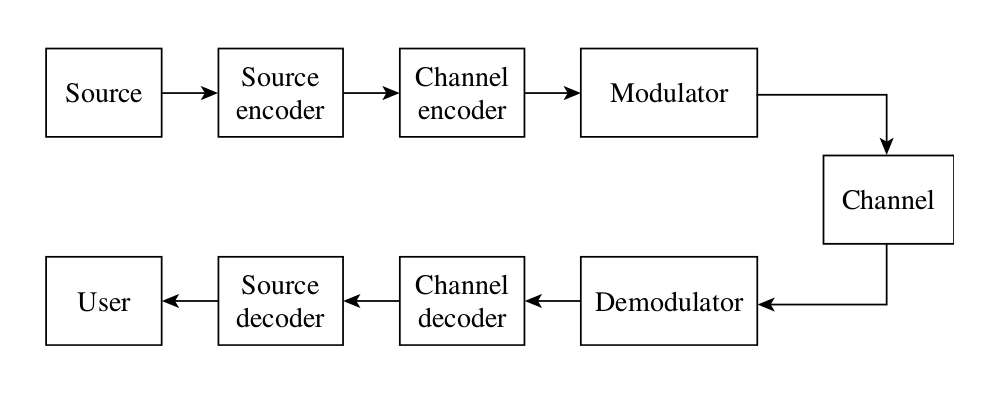
\includegraphics[width=0.8\linewidth]{figures/comm_system_2.png}}
\caption{Κύρια μέρη του τηλεπικοινωνιακού συστήματος}
\label{fig:telecom system 2}
\end{figure}

\subsection*{Το κανάλι}
Σε αυτό το σημείο θα γίνει μια συνοπτική παρουσίαση του τηλεπικοινωνιακού καναλιού. Tο τηλεπικοινωνιακό κανάλι ορίζεται ως ο χώρος που μεσολαβεί ανάμεσα στον πομπό και τον δέκτη και στον οποίο λαμβάνει χώρα η μετάδοση πληροφορίας. Σε θεωρητικό επίπεδο, το κανάλι αποτελεί τη μαθηματική αφαίρεση των ειδών και της έντασης του θορύβου που αλλοιώνει τη μεταδιδόμενη πληροφορία.
\begin{figure}[h]
\center{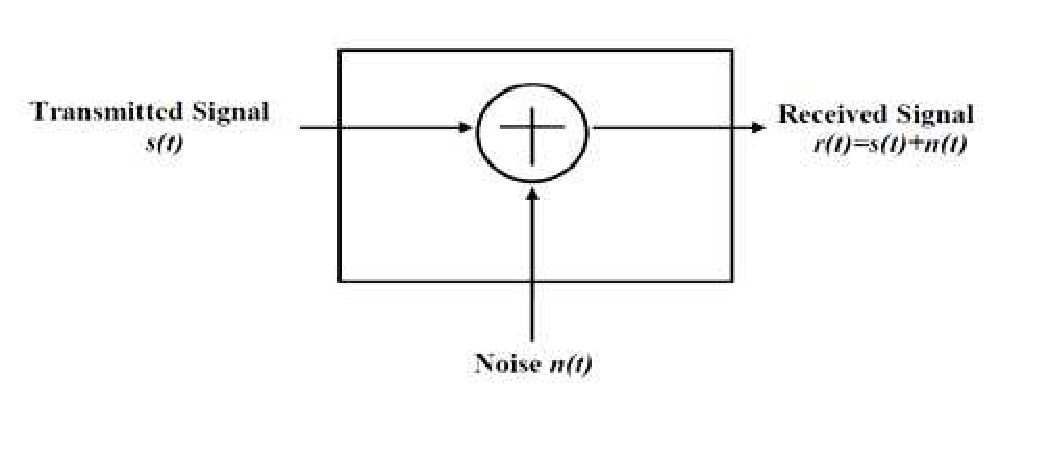
\includegraphics[width=0.8\linewidth]{figures/awgn_channel.eps}}
\caption{Κανάλι \en{AWGN} θορύβου}
\label{fig:awgn channel}
\end{figure}

Όπως φαίνεται στο Σχήμα \ref{fig:awgn channel}, στο μεταδιδόμενο σήμα $s(t)$ προστίθεται ο θόρυβος που εισάγεται κατά τη μετάδοση από το κανάλι και αποτελεί αναπόδραστη αιτία υποβάθμισης του σήματος πληροφορίας. Ο θόρυβος εκτός από προσθετικός, μοντελοποιείται ως λευκός (ίση πυκνότητα ισχύος σε όλο το φάσμα συχνοτήτων), \en{Gaussian} (ακολουθεί την κανονική ή γκαουσσιανή κατανομή στο πεδίο του χρόνου) θόρυβος (\en{Additive White Gaussian Noise, AWGN)}.

\vspace{5mm}

Στην περίπτωση που η είσοδος του καναλιού αποτελεί μια διακριτή ακολουθία, το κανάλι καλείται \textit{διακριτό} (\en{discrete channel}) και ορίζεται ως εξής:

\begin{definition}
Το διακριτό κανάλι, συμβολιζόμενο ως ($\mathcal{X},\;p(x\mid{y}),\;\mathcal{Y}$), αποτελείται από δύο πεπερασμένα σύνολα (\en{finite sets}) $\mathcal{X}$ και $\mathcal{Y}$, καθώς και μια συλλογή συναρτήσεων πυκνότητας πιθανότητας $p(x\mid{y})$, μία για κάθε $x\in\mathcal{X}$, τέτοιες ώστε, για κάθε $x$, $y$ να ισχύει $p(y\mid{x})\ge0$ και $\sum\nolimits_{y}p(y\mid{x})=1\;\;\forall{x}$, όταν $\mathcal{X}$ είναι η είσοδος και $\mathcal{Y}$ η έξοδος του καναλιού \cite{cover2012elements}.
\label{def:discrete channel}
\end{definition}

\en{\lipsum[1]}

\section{Θεώρημα \en{Shannon}}
Για κάθε τηλεπικοινωνιακό σύστημα, ισχύει το παρακάτω θεώρημα, το οποίο  αποτελεί θεμελιώδες θεώρημα της θεωρίας τηλεπικοινωνιών:
\begin{theorem}(Θεώρημα Κωδικοποίησης Ενθόρυβου Καναλιού)
Ο ρυθμός αποστολής πληροφορίας μέσω του τηλεπικοινωνιακού συστήματος έχει μέγιστο \en{C}, που καλείται \textbf{χωρητικότητα καναλιού}
\begin{itemize}
\item Όταν ισχύει:
\begin{equation}
R\leq{C}
\end{equation}
,όπου $R$ ο ρυθμός αποστολής της πληροφορίας (\en{bits} ανά χρήση του καναλιού), τότε υπάρχει τεχνική κωδικοποίησης καναλιού, έτσι ώστε να είναι δυνατή μετάδοση με αυθαίρετα μικρό σφάλμα.
\item Στην αντίθετη περίπτωση η αξιοπιστία της επικοινωνίας δεν μπορεί να ελεγχθεί.
\end{itemize}
\label{theorem:shannon}
\end{theorem}

\en{\lipsum[1]}

Αξίζει να σημειωθεί πως, ενώ το θεώρημα \en{Shannon} αποδεικνύει, για οποιοδήποτε ρυθμό μικρότερο της χωρητικότητας την ύπαρξη τεχνικών κωδικοποίησης, κατάλληλων ώστε να υπάρχει οσοδήποτε μικρό σφάλμα κατά την επικοινωνία, η απόδειξη δεν είναι κατασκευαστική (\en{constructive}), δηλαδή δεν προτείνεται κάποιος συγκεκριμένος κώδικας \cite{shannon1948mathematical}.

Στη συνέχεια θα οριστεί ένας τυχαίος κώδικας που ικανοποιεί το Θεώρημα \ref{theorem:shannon} και θα εξεταστεί ο τρόπος κατασκευής του και η πολυπλοκότητα την οποία εισάγει η χρήση του.

\section{Τυχαίοι κώδικες - Πολυπλοκότητα}
\begin{definition}{Κώδικας $C(n,M)$}

Ένας κώδικας $C(n,M)$ για ένα διακριτό κανάλι που προκύπτει από τον Ορισμό \ref{def:discrete channel}, αποτελείται από τα εξής στοιχεία:
\begin{itemize}
\item Ένα σύνολο δεικτών $[1, 2, \ldots, M]$ 
\item Μια συνάρτηση κωδικοποίησης $X^n:\left\lbrace1, 2, \ldots, M\right\rbrace\to\mathcal{X}^n$ η οποία παράγει τις κωδικές λέξεις $x^n\left(1\right), x^n\left(2\right), \ldots, x^n\left(M\right)$. Το σύνολο των κωδικών λέξεων, καλείται \textit{κωδικό βιβλίο}
\item Μια συνάρτηση αποκωδικοποίησης $g:\mathcal{Y}^n\to\left\lbrace1, 2, \ldots, M\right\rbrace$ η οποία λειτουργεί ως ένας ντετερμινιστικός κανόνας, που αποδίδει μια πρόβλεψη σε κάθε ληφθέν διάνυσμα
\end{itemize}
Στο εξής, όταν αναφέρεται κώδικας, θα εννοείται το κωδικό βιβλίο του, το οποίο θα συμβολίζεται ως $C(n,M)$.
\label{def:code}
\end{definition}

Χρησιμοποιώντας τη σημειολογία του ορισμού \ref{def:code}, ο \textit{ρυθμός κώδικα} $C(n,M)$ (ρυθμός αποστολής πληροφορίας) ορίζεται από την παρακάτω εξίσωση:
\begin{equation}
R=\frac{\log_{2}M}{n}\;\;\;\;(bits/transmission)
\label{eq: code rate}
\end{equation}
\cite{cover2012elements}.

Θα χρειαστεί να σημειωθεί, όπως αναφέρθηκε και στην προηγούμενη παράγραφο πως, ενώ το θεώρημα \en{Shannon} αποδεικνύει την ύπαρξη κωδίκων που πλησιάζουν τη χωρητικότητα, δεν προτείνει κάποια συγκεκριμένη επιλογή βέλτιστου κώδικα. Η ρητή κατασκευή (\en{explicit construction}) \enquote*{καλών} κωδίκων αποτελεί δύσκολο έργο.

Αντί αυτής, η τυπική προσέγγιση βασίζεται στην πιθανοτική μέθοδο (\en{probabilistic method}) και προβλέπει πως σε ένα σύνολο κωδίκων οι οποίοι έχουν κατασκευαστεί με τυχαίο τρόπο, η πιθανότητα να υπάρχουν καλοί κώδικες εντός του είναι θετική. Για την ακρίβεια, κάνοντας χρήση κάποιας ανισότητας συγκέντρωσης (π.χ. ανισότητα \en{Markov}), αποδεικνύεται πως η πιθανότητα να επιλεγεί ένας καλός κώδικας μέσα από αυτό το σύνολο τείνει στο 1, καθώς το μήκος του κώδικα $n$ μεγαλώνει.

\subsection{Τυχαίοι κώδικες}
\en{\lipsum[1]}



Ένα σώμα πεπερασμένου αριθμού στοιχείων (\en{finite field}) $\mathbb{F}_q$, είναι ένα σύνολο από στοιχεία των οποίων το άθροισμα και το γινόμενο, είναι επίσης στοιχεία του συνόλου. Επίσης, η πρόσθεση κι ο πολλαπλασιασμός στοιχείων ικανοποιούν την αντιμεταθετική, προσεταιριστική, και επιμεριστική ιδιότητα. Tο πλήθος των στοιχείων ενός σώματος συμβολίζεται ως $|\mathbb{F}_q|$. Ευρέως χρησιμοποιούμενο είναι το \textit{δυαδικό} σώμα $\mathbb{F}_2$ το οποίο αποτελείται από τα στοιχεία \{0,1\}, επομένως ισχύει $|\mathbb{F}_2|=2$. Το σώμα αυτό θα υποθέτουμε και σε όλη την έκταση της παρούσας εργασίας.

Η κατασκευή τυχαίων κωδίκων επί του σώματος $\mathbb{F}_2$, ακολουθεί την εξής διαδικασία:
\begin{definition}{(Τυχαίο σύνολο \en{Shannon}).}

Το σύνολο όλων των κωδίκων $C(n,M)$ μήκους $n$ και πληθυκότητας $M$ αποτελείται από $|\mathbb{F}|_2^{nM}$ δυνατούς κώδικες, καθώς υπάρχουν $nM$ βαθμοί ελευθερίας στην επιλογή κάθε στοιχείου του κωδικού βιβλίου. Στα στοιχεία του συνόλου προσδίδεται η ομοιόμορφη κατανομή πιθανότητας και επιλέγονται τυχαία τα στοιχεία $x^{[1]},...,x^{[M]}$ του συνόλου. \cite{richardson2008modern},\cite{shannon1948mathematical}
\label{def:random_ensemble}
\end{definition}

\en{\lipsum[1]}
\subsection{Πολυπλοκότητα}
Είναι προφανές πως, οι (τυχαίοι) κώδικες που προκύπτουν από τον Ορισμό \ref{def:random_ensemble} ικανοποιούν και το θεώρημα \en{Shannon}, είναι δηλαδή ικανοί να λειτουργήσουν κοντά στη χωρητικότητα, με αυθαίρετα μικρό σφάλμα. Παρά το ότι η τυχαία κωδικοποίηση αποτελεί την προφανή λύση στο πρόβλημα κωδικοποίσης, υστερεί σε δυνατότητα πρακτικής υλοποίησης, καθώς δεν λαμβάνει υπ'όψιν την πολυπλοκότητα αποθήκευσης του κώδικα (πολυπλοκότητα περιγραφής) και την πολυπλοκότητα κωδικοποίησης και αποκωδικοποίησης.

Στην περίπτωση ενός κώδικα που προκύπτει από τον Ορισμό \ref{def:random_ensemble}, προκύπτει εύκολα πως η πολυπλοκότητα αποθήκευσης είναι εκθετική με το μήκος του κώδικα, καθώς απαιτούνται $nM = n\*2^{Rn}$ \en{bits} για την αποθήκευση του κωδικού βιβλίου $C(n,M)$ στον κωδικοποιητή, για τη σύνθεση του μηνύματος που θα εισέλθει για μετάδοση από το κανάλι. Ακόμη ο αποκωδικοποιητής θα πρέπει να έχει αποθηκευμένη κάθε δυνατή κωδική λέξη και (όπως ήδη αναφέρθηκε) να εκτελέσει αναζήτηση για τον έλεγχο και την απόφαση του μηνύματος πληροφορίας που στάλθηκε. Παρατηρείται συνεπώς, πως με την αύξηση του μήκους \en{n} η πολυπλοκότητα καθίσταται απαγορευτική. 

Συνοψίζοντας, διαπιστώνεται πως το πρόβλημα έγκειται στη δυνατότητα προσέγγισης της χωρητικότητας με πρακτικό τρόπο.
 
\subsection{Πρακτικοί κωδικοποιητές/αποκωδικοποιητές}
Τη δυνατότητα αυτοί δίνουν διαδικασίες κωδικοποίησης (\en{coding schemes}) και αποκωδικοποίσης, σχεδιασμένες με γνώμονα τη δυνατότητα πρακτικής υλοποίησης. Οι κώδικες που προκύπτουν διακρίνονται από δομικές αλγεβρικές ιδιότητες και ορίζονται από συγκεκριμένους κανόνες για την κωδικοποίηση και την αποκωδικοποίηση.

Θα αποδειχθεί στη συνέχεια της εργασίας, πως με έναν τέτοιο τρόπο, η πολυπλοκότητα κωδικοποίησης και αποκωδικοποίησης απλοποιείται σημαντικά, και καταλήγει να είναι τετραγωνικής ($\mathcal{O}(n^2)$) ή και γραμμικής ($\mathcal{O}(n)$) τάξης.Οι αλγεβρικές δομικές ιδιότητες προσδίδονται στους κώδικες για ακριβώς το σκοπό αυτό. Θα οριστούν επίσης έννοιες όπως οι αραιοί πίνακες, η επαναληπτική αποκωδικοποίηση και τα γραφήματα \en{Tanner} ως εργαλεία για την περιγραφή τέτοιων κωδίκων.

\section{Δομή εργασίας}
Η εργασία θα ακολουθήσει την εξής δομή: Στο Κεφάλαιο 2 θα αναλυθούν οι αλγεβρικές δομικές ιδιότητες των κωδίκων καναλιού, ώστε να καταστεί πρακτική η κωδικοποίηση και αποκωδικοποίηση τους και θα οριστούν οι γραμμικοί μετασχηματισμοί για την εκτέλεσή τους, οι πίνακες \textbf{\en{G}} και \textbf{\en{H}}. Στο Κεφάλαιο 3 θα οριστούν και θα περιγραφούν οι κώδικες επανάληψης - συσσώρευσης (\en{repeat-accumulate}) ως υποομάδα τόσο των κωδίκων \en{turbo} όσο και των \en{LDPC} κωδίκων και θα εξεταστεί ο μηχανισμός και η πολυπλοκότητα κωδικοποίησης και αποκωδικοποίησής τους. Στο Κεφάλαιο 4 θα περιγραφεί αναλυτικά η προσομοίωση που έγινε και θα παρουσιαστούν τα αποτελέσματά της. Τέλος στο Κεφάλαιο 5 θα παρουσιαστούν οι δυνατότητες περαιτέρω μελέτης καθώς και πρόσθετες επεκτάσεις, στηριζόμενες στη γλωσσα \en{C}\texttt{++} και \en{CUDA C}.
	\chapter{\selectlanguage{greek}Γραμμικοί Μπλoκ Κώδικες}\externaldocument{chapter1.tex}
Στο κεφάλαιο αυτό, παρουσιάζονται οι βασικές αλγεβρικές δομικές ιδιότητες που προσδίδονται στους κώδικες καναλιού οι οποίες διακρίνουν τους κώδικες πάνω στους οποίους στηρίζεται η παρούσα εργασία και που θα παρουσιαστούν στο επόμενο κεφάλαιο. Όπως αναφέρθηκε στο εισαγωγικό κεφάλαιο, θεωρείται πως η έξοδος της πηγής πληροφορίας είναι μια διακριτή ακολουθία δυαδικών ψηφίων, η οποία καλείται \textit{ακολουθία πληροφορίας}. Η μετάδοση λαμβάνει χώρα μέσω του διακριτού καναλιού, όπως αυτό ορίστηκε στον Ορισμό \ref{def:discrete channel}. Υπενθυμίζεται ακόμη πως η έκφραση \enquote{κώδικας $C(n,M)$}, αναφέρεται στο κωδικό βιβλίο του κώδικα και το σώμα που υποθέτουμε είναι το $\mathbb{F}_2$.

\section{\en{Block} κώδικες}
Ξεκινώντας, οι κώδικες καναλιού, μπορούν να διαχωριστούν σε 2 υποομάδες, τους \textit{συνελικτικούς} κώδικες (\en{convolutional codes}) και τους κώδικες \textit{\en{block}} (\en{block codes}).

Η αρχή λειτουργίας της \en{block} κωδικοποίησης, συνίσταται στην κατάτμηση της ακολουθίας πληροφορίας σε σταθερά \en{block} $\mathbf{u} = (u_0, u_1, ..., u_{k-1})$ μήκους $k$ και στην απεικόνισή της στην είσοδο του καναλιού στην κωδική λέξη $\mathbf{v} = (v_0, v_1, ..., v_{n-1})$ μήκους $n$, με $n>k$, μέσω κάποιων συγκεκριμένων κανόνων. H απεικόνιση αυτή είναι ανεξάρτητη από τα προηγούμενα \en{block}, δηλαδή δεν υπάρχει μνήμη από ένα \en{block} μήνυμα, σε ένα άλλο επόμενο \cite{proakis1994communication}.

\begin{figure}[h]
\center{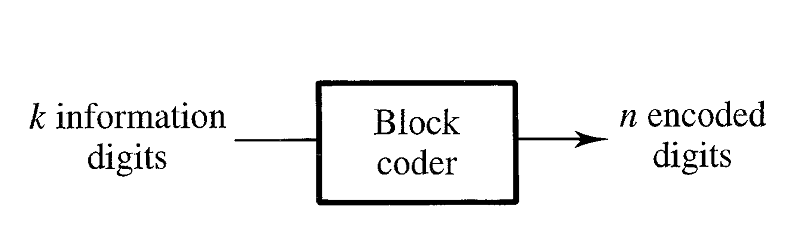
\includegraphics[width=0.75\linewidth]{figures/linear_block_codes.png}}
\caption{Σχηματικό διάγραμμα ενός \en{block} κώδικα}
\label{fig:linear block codes}
\end{figure}

\subsection{Ρυθμός κώδικα}
Στο προηγούμενο κεφάλαιο ορίστηκε ο ρυθμός του κώδικα ως $R=\frac{\log_{2}M}{n}$. Επίσης ισχύει πως η πληθυκότητα (\en{cardinality}) του \en{block} κώδικα $C$ στο $\mathbb{F}_2$, το σύνολο δηλαδή των δυνατών κωδικών λέξεων του κωδικού βιβλίου, είναι $M=2^k$. Εφαρμόζοντας τις παραπάνω σχέσεις, προκύπτει ο λόγος
\begin{equation}
R = \frac{\log_{2}2^{k}}{n} = \frac{k}{n}
\label{eq:code rate}
\end{equation}
ο οποίος καλείται \textit{ρυθμός} του \en{block} κώδικα $C$ (\en{\textit{code rate}}) και αντιπροσωπεύει τον μέσο όρο πληροφορίας που αποστέλλεται με κάθε κωδικό \en{bit}, ανν τα \en{bits} πληροφορίας είναι ανεξάρτητα και ισοπίθανα (\en{i.i.d.}). Προφανώς ισχύει $0<R<1$.

\vspace{5mm}

Όπως αναφέρθηκε, ο κώδικας αντιστοιχίζει κάθε μήνυμα πληροφορίας $\mathbf{u}$, στην κωδικολέξη $\mathbf{v}$, μήκους $n$, με $n>k$. Tα $n-k$ επιπλέον \en{bits} που προστίθενται στο μήνυμα από τον κωδικοποιητή καναλιού καλούνται \textit{πλεονασματικά} (\en{\textit{redundant bits}}).

Τα πλεονασματικά \en{bits} δεν περιέχουν επιπλέον πληροφορία και ο σκοπός τους είναι να δώσουν δυνατότητες \textit{ανίχνευσης} και \textit{διόρθωσης} σφαλμάτων, που προκύπτουν κατά τη μετάδοση στο κανάλι, λόγω θορύβου ή/και παρεμβολών. Το πως διαμορφώνονται αυτά τα πλεονασματικά \en{bits}, ώστε ο \en{block} κώδικας $C(n,k)$ να έχει ικανοποιητικές δυνατότητες ανίχνευσης ή/και διόρθωσης, αποτελεί μείζων ζήτημα της σχεδίασης μηχανισμών κωδικοποίησης \cite{ryan2009channel}.

\section{Γραμμικοί \en{block} κώδικες}
Για ένα \en{block} κώδικα $C(n,M)$, με $2^k$ κωδικές λέξεις και χωρίς περεταίρω δομή, έχει ήδη αναφερθεί πως ο μηχανισμός κωδικοποίησης απαιτείται να καταχωρεί τις $2^k$ κωδικές αυτές λέξεις σε ένα κωδικό λεξικό και ο μηχανισμός αποκωδικοποίησης να κάνει αναζήτηση σε ένα πίνακα $2^k\times{n}$, ώστε να αποφασίσει για τη μεταδιδόμενη κωδική λέξη.

Επομένως, επιπρόσθετα από την δόμηση σε κωδικά \en{blocks}, είναι αναγκαίο να προσδώσουμε επιπλέον ειδικές αλγεβρικές δομικές ιδιότητες στον κώδικα $C(n,M)$, ώστε οι παραπάνω διαδικασίες να καταστούν πρακτικά υλοποιήσιμες. Μια τέτοια επιθυμητή δομική ιδιότητα ώστε ο \en{block} κώδικας να είναι υλοποιήσιμος με πρακτικό τρόπο, είναι η \textit{γραμμικότητα}.

\begin{definition}
Ένας δυαδικός κώδικας μήκους $n$ καλείται $(n,k)$ \textit{γραμμικός \en{block} κώδικας}, ανν οι $2^k$ κωδικές του λέξεις σχηματίζουν έναν $k$-διάστατο υποχώρο του δυανυσματικού χώρου $V$ όλων των δυνατών $n$-άδων στο $\mathbb{F}_2$ \cite{ryan2009channel}.
\label{def:linear block code}
\end{definition}

Ένας ισοδύναμος ορισμός είναι ο εξής:

\begin{definition}
Ένας κώδικας \en{block} είναι γραμμικός αν κάθε γραμμικός συνδυασμός δύο κωδικών του λέξεων, είναι επίσης κωδική του λέξη. Στο $\mathbb{F}_2$, αν $\mathbf{c_i}$ και $\mathbf{c_j}$ οι δύο κωδικές λέξεις, τότε πρέπει $\mathbf{c_i}\oplus\mathbf{c_j}$ να είναι επίσης κωδική λέξη του $C$, όπου με $\oplus$ συμβολίζεται η συνιστώσα-προς-συνιστώσα \en{modulo-2} πρόσθεση \cite{proakis1994communication}.
\end{definition}

Φαίνεται επομένως πως ένας (δυαδικός) \en{block} κώδικας είναι γραμμικός, ανν υπάρχει \enquote*{1-1} αντιστοιχία μεταξύ του μηνύματος \en{\textbf{u}} και της κωδικολέξης \en{\textbf{v}}. Επίσης, η ακολουθία \textbf{0} αποτελεί κωδική λέξη κάθε γραμμικού \en{block} κώδικα, αφού μπορεί να προκύψει ως συνιστώσα-προς-συνιστώσα \en{modulo-2} πρόσθεση μιας κωδικής λέξης με τον εαυτό της. Ακόμη φαίνεται πως η γραμμικότητα ενός κώδικα εξαρτάται αποκλειστικά από τις κωδικές του λέξεις και όχι από τον τρόπο με τον οποίο η ακολουθία πληροφορίας απεικονίζεται σε αυτές.

\section{Αναπαράσταση σε πίνακα}

\subsection{Πίνακας \en{G}}
Σύμφωνα με τον ορισμό του γραμμικού \en{block} κώδικα $C(n,k)$, αποδεικνύεται πως υπάρχουν $k$ γραμμικά ανεξάρτητες κωδικές λέξεις, $\mathbf{g_0, g_1, ..., g_{k-1}}$, έτσι ώστε κάθε κωδική λέξη $\mathbf{v}$ να προκύπτει ως γραμμικός συνδυασμός τους. Οι $k$ γραμμικά ανεξάρτητες αυτές κωδικές λέξεις λέγεται ότι σχηματίζουν μια \textit{βάση} του $C$.

Με βάση αυτό, η κωδική λέξη προκύπτει ως εξής: έστω $\mathbf{u} = (u_0, u_1, ..., u_{k-1})$ το μήνυμα στην είσοδο του κωδικοποιητή. Η κωδικολέξη $\mathbf{v} = (v_0, v_1, ..., v_{n-1})$ δίνεται από τον γραμμικό συνδυασμό των $\mathbf{g_0, g_1, ..., g_{k-1}}$ με συντελεστές τα $k$ \en{bits} πληροφορίας, από την παρακάτω εξίσωση:

\begin{equation}
\mathbf{v}=u_0\mathbf{g_0}+u_1\mathbf{g_1}+...+u_{k-1}\mathbf{g_{k-1}}
\label{eq:codeword formation}
\end{equation}

Οι συνιστώσες των $k$ γραμμικά ανεξάρτητων κωδικολέξεων μπορούν να αναπαρασταθούν ως γραμμές ενός $k\times n$ πίνακα στο $\mathbb{F}_2$ ως εξής:

\begin{equation}
\mathbf{G}=\begin{bmatrix}\mathbf{g_0}\\\mathbf{g_1}\\\vdots\\\mathbf{g_{k-1}}\\\end{bmatrix}=\begin{bmatrix}g_{0,0} & g_{0,1} & \cdots & g_{0,n-1}\\g_{1,0} & g_{1,1} & \cdots & g_{1,n-1}\\\vdots & \vdots & \ddots & \vdots\\g_{k-1,0} & g_{k-1,1} & \cdots & g_{k-1,n-1}\\\end{bmatrix}
\label{eq:generator matrix}
\end{equation}

Σε αυτή την περίπτωση, η κωδικολέξη $\mathbf{v}$ που αντιστοιχεί στο μήνυμα $\mathbf{u}$, δίνεται από τον πολλαπλασιασμό πινάκων: 

\begin{equation}
\mathbf{v=u \cdot G}
\label{eq:check equation}
\end{equation}

Ο πίνακας \en{\textbf{G}} καλείται \textit{πίνακας γεννήτορας} \en{(generator matrix)} του $(n,k)$ γραμμικού \en{block} κώδικα $C$. Γενικά, ένας γραμμικός \en{block} κώδικας δεν έχει μοναδική βάση. Συνεπώς κάθε επιλογή βάσης του $C$ δίνει διαφορετικό γεννήτορα πίνακα, οπότε προκύπτει πως ο πίνακας \en{\textbf{G}} δεν είναι μοναδικός για δεδομένο κώδικα. Ο βαθμός (\en{rank}) του πίνακα \en{\textbf{G}} είναι προφανώς ίσος με τη διάσταση του κώδικα $C$.

Μειώνεται συνεπώς σημαντικά η πολυπλοκότητα περιγραφής του κώδικα, αφού πλέον αρκέι ο κωδικοποιητής να αποθηκεύσει τις $k$ γραμμές του πίνακα \en{\textbf{G}}. Επιπρόσθετα, η εκτέλεση του πολλαπλασιασμού που περιγράφει η \ref{eq:check equation} απαιτεί περίπου $kn$ πράξεις, δηλαδή είναι τετραγωνικής πολυπλοκότητας ως προς το $n$ - $\mathcal{O}(n^2)$.

\subsection{Πίνακας \en{H}}
\begin{definition}
Ο δυικός κώδικας (\en{\textit{dual code}}) του $C$, $C_d$ δίνεται από τις παρακάτω $n$-άδες:$$C_d=\lbrace\mathbf{w}\in V:\langle \mathbf{w,v} \rangle =0\;\;\;\forall\;\mathbf{v}\in C\rbrace$$,
όπου με $\langle\cdot,\cdot\rangle$ συμβολίζεται το διανυσματικό εσωτερικό γινόμενο \cite{ryan2009channel}.
\label{def:dual code}
\end{definition}

Από τον Ορισμό \ref{def:dual code} προκύπτουν τα παρακάτω:

\begin{itemize}
\item Αν η βάση του $C$ αποτελείται από $k$ γραμμικά ανεξάρτητες κωδικές λέξεις, η βάση του $C_d$ αποτελείται από ($n-k$) γραμμικά ανεξάρτητες $n$-άδες.
\item Έστω $\mathbf{h_0, h_1, ..., h_{n-k-1}}$ οι ($n-k$) γραμμικά ανεξάρτητες $n$-άδες. Συνεπάγεται πως κάθε $n$-άδα στον $C_d$ προκύπτει ως γραμμικός συνδυασμός τους
\item Ομοίως με τον πίνακα \en{\textbf{G}}, οι παραπάνω γρ. ανεξάρτητες $n$-άδες μπορούν να αναπαρασταθούν ως γραμμές ενός πίνακα στο $\mathbb{F}_2$, που σχηματίζεται ως εξής:

\begin{equation}
\mathbf{H}=\begin{bmatrix}\mathbf{h_0}\\\mathbf{h_1}\\\vdots\\\mathbf{h_{n-k-1}}\\\end{bmatrix}=\begin{bmatrix}h_{0,0} & h_{0,1} & \cdots & h_{0,n-1}\\h_{1,0} & h_{1,1} & \cdots & h_{1,n-1}\\\vdots & \vdots & \ddots & \vdots\\h_{n-k-1,0} & h_{n-k-1,1} & \cdots & h_{n-k-1,n-1}\\\end{bmatrix}
\label{eq:parity check matrix}
\end{equation}
\item Ο πίνακας $\mathbf{H}$ είναι γεννήτορας πίνακας του $C_d$, ακριβώς όπως ο $\mathbf{G}$ είναι του $C$. Λόγω αυτού και από την ιδιότητα της ορθογωνιότητας, προκύπτει η πολύ χρήσιμη εξίσωση $\mathbf{G} \cdot \mathbf{H^T} = \mathbf{0}$, όπου $\mathbf{0}$ μηδενικός $k \times (n-k)$ πίνακας.
\end{itemize}

Ακόμη προκύπτει πως ο κώδικας $C$ ορίζεται με μοναδικό τρόπο από τον πίνακα $\mathbf{H}$, επειδή κάθε δυαδική $n$-άδα $\mathbf{v}$ είναι κωδικολέξη του $C$ ανν
ισχύει $\mathbf{v} \cdot \mathbf{H^T} = \mathbf{0}$, δηλαδή
\begin{equation}
C=\lbrace\mathbf{v}\in V:\mathbf{v} \cdot \mathbf{H^T} = \mathbf{0}\rbrace
\label{eq:decoding equation}
\end{equation}

Ο πίνακας $\mathbf{H}$ καλείται πίνακας \textit{ελέγχου ισοτιμίας} (\en{parity check matrix}) του κώδικα $C$. Από την παραπάνω σχέση ορισμού ενός γραμμικού κώδικα (Σχέση \ref{eq:decoding equation}), προέρχεται και το όνομα του $\mathbf{H}$, αφού, στην πλευρά του αποκωδικοποιητή, ο $\mathbf{H}$ χρησιμοποιείται για την επαλήθευση του παραπάνω συστήματος ομογενών εξισώσεων, όταν το διάνυσμα $\mathbf{v}$, αντικατασταθεί με το ληφθέν διάνυσμα.

Παρατηρείται επομένως, πως ο γραμμικός \en{block} κώδικας $C$ μπορεί να οριστεί πλήρως από δύο πίνακες, τον γεννήτορα και τον πίνακα ελέγχου ισοτιμίας. Στη γενική περίπτωση, η κωδικοποίηση του $C$ βασίζεται στον γεννήτορα πίνακα και ακολουθεί την εξίσωση \ref{eq:check equation}, ενώ η αποκωδικοποίηση βασίζεται στον πίνακα ελέγχου ισοτιμίας.

Ο πίνακας ελέγχου ισοτιμίας μπορεί να περιγράψει πλήρως έναν κώδικα, και πολλές κατηγορίες γραμμικών \en{block} κωδίκων κατασκευάζονται με βάση τον πίνακα $\mathbf{H}$. Ο πίνακας $\mathbf{H}$ είναι σε μορφή \textit{πλήρους βαθμού} (\en{full rank}), ανν ο βαθμός του είναι ίσος με το πλήθος των σειρών. Σε πολλές περιπτώσεις, ο πίνακας $\mathbf{H}$ δεν δίνεται σε \en{full rank} μορφή, δηλαδή το πλήθος των σειρών του είναι μεγαλύτερο από το \en{rank} του, $n-k$, ή ισοδύναμα, ορισμένες από τις σειρλες είναι γραμμικός συνδυασμός των $n-k$ γραμμικά ανεξάρτητων σειρών. Οι σειρές αυτές ονομάζονται \textit{πλεονάζουσες} (\en{redundant}) σειρές. 

Οι κώδικες Πίνακα Ισοτιμίας Χαμήλης Πυκνότητας (\en{Low Density Parity Check - LDPC}), που θα εξεταστούν στη συνέχεια της εργασίας, διακρίνονται από πίνακες $\mathbf{H}$ που δεν είναι \en{full rank} \cite{cover2012elements}, \cite{ryan2009channel}.

\section{Κώδικες σε συστηματική μορφή}

\begin{figure}[h]
\center{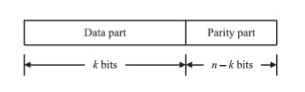
\includegraphics[width=0.65\linewidth]{figures/systematic_form.png}}
\caption{Κωδική λέξη σε συστηματική μορφή}
\label{fig:systematic form}
\end{figure}

Είναι επίσης επιθυμητό, οι κωδικές λέξεις ενός γραμμικού \en{block} κώδικα $C(n,k)$ να έχουν τη μορφή που φαίνεται στο Σχήμα \ref{fig:systematic form}, η οποία καλείται \textit{συστηματική μορφή}. Στη συστηματική μορφή, η κωδική λέξη χωρίζεται στο τμήμα μηνύματος (\en{data part}) και στο πλεονάζον τμήμα ελέγχου (\en{parity part}). Το τμήμα μηνύματος αποτελείται από τα $k$ αναλλοίωτα ψηφία πληροφορίας και το πλεονάζον τμήμα ελέγχου, από τα $n-k$ \en{bits} ελέγχου ισοτιμίας. Ολόκληρος ο γραμμικός \en{block} κώδικας $C(n,k)$ βρίσκεται σε \textit{συστηματική} μορφή, όταν όλα τα στοιχεία του κωδικού βιβλίου βρίσκονται σε συστηματική μορφή, ή ισοδύναμα, όταν μπορέι να οριστεί πλήρως από έναν $k \times n$ γεννήτορα πίνακα με την παρακάτω μορφή:

\begin{equation}
\mathbf{G} = \left[\mathbf{P}\;\;\mathbf{I}_{k}\right]= 
\left[\underbrace{\begin{matrix}
p_{0,0} & p_{0,1} & \cdots & p_{0,n-k-1} \\
p_{1,0} & p_{1,1} & \cdots & p_{1,n-k-1} \\
\vdots & \vdots & \ddots & \vdots \\
p_{k-1,0} & p_{k-1,1} & \cdots & p_{k-1,n-k-1}
\end{matrix}}_{\text{\en{\textbf{P}} πίνακας}}\;
\underbrace{\begin{matrix}
1 & 0 & \cdots & 0 \\
0 & 1 & \cdots & 0 \\
\vdots & \vdots & \ddots & \vdots \\
0 & 0 & \cdots & 1
\end{matrix}}_{\text{$k\times k$ $\mathbf{I}_k$ μοναδιαίος πίνακας}}\right]
\label{eq:generator matrix systematic form}
\end{equation}

\vspace{5mm}

Όπως διαπιστώνεται και από την εξίσωση \ref{eq:generator matrix systematic form}, ο γεννήτορας πίνακας $\mathbf{G}$, που για συντομία σημειώνεται ως $\mathbf{G}=\left[\mathbf{P}\;\;\mathbf{I}_k\right]$, αποτελείται από δύο υποπίνακες, έναν $k\times (n-k)$ υποπίνακα $\mathbf{P}$ στα αριστερά, ο οποίος καλείται υποπίνακας ελέγχου ισοτιμίας του $\mathbf{G}$ και έναν $k\times k$ μοναδιαίο πίνακα $\mathbf{I}_k$ στα δεξιά \cite{ryan2009channel}.

Η συστηματική μορφή του πίνακα $\mathbf{G}$ έχει σημαντικά πλεονεκτήματα καθώς σε κάθε κωδική λέξη, τα \en{bits} πληροφορίας παραμένουν αναλλοίωτα στις αρχικές $k$ θέσεις της. Μειώνεται συνεπώς η πολυπλοκότητα κωδικοποίησης, αφού χρειάζεται να υπολογιστούν μόνο τα σύμβολα στις θέσεις του πλεονάζοντος τμήματος ελέγχου.

Αντίστοιχα, η συστηματική μορφή του πίνακα ελέγχου ισοτιμίας διαμορφώνεται ως εξής:

\begin{equation}
\mathbf{H}=\left[\mathbf{I}_{n-k}\;\;\mathbf{P^T}\right]
=\begin{bmatrix}
1 & 0 & \cdots & 0 & \; & p_{0,0} & p_{1,0} & \cdots & p_{k-1,0} \\
0 & 1 & \cdots & 0 & \; & p_{0,1} & p_{1,1} & \cdots & p_{k-1,1} \\
\vdots & \vdots & \ddots & \vdots  & \; & \vdots & \vdots & \ddots & \vdots \\
0 & 0 & \cdots & 1 & \; & p_{0,n-k} & p_{1,n-k} & \cdots & p_{k-1,n-k}
\end{bmatrix}
\label{eq:parity check matrix systematic form}
\end{equation}

\vspace{5mm}
Προφανώς ισχύει και πάλι ότι $\mathbf{G}\cdot\mathbf{H^T}=\mathbf{0}$.

Θεωρείται και πάλι το μήνυμα πληροφορίας $\mathbf{u} = (u_0, u_1, ..., u_{k-1})$. Αν εφαρμοστεί η εξίσωση \ref{eq:check equation}, όταν ο πίνακας $\mathbf{G}$ είναι σε συστηματική μορφή, η κωδική λέξη προκύπτει από τον παρακάτω πολλαπλασιασμό:

\begin{equation}
\begin{split}
\mathbf{v} & = \left( u_0, u_1, \cdots, u_{k-1} \right) \cdot \mathbf{G}\\
& = \left( v_0, v_1, \cdots, v_{n-k-1}, v_{n-k}, \cdots, v_{n-1} \right)
\end{split}
\label{eq:systematic codeword formation}
\end{equation}

\vspace{5mm}

τα $n$ στοιχεία της οποίας προκύπτουν ως εξής:

\begin{equation}
\begin{aligned}
v_{n-k+i}=u_i\;\;\ & \forall\;\;0\leq i < k  \\
v_j=u_0p_{0,j}+u_1p_{1,j}+\cdots+u_{k-1}p_{k-1,j}\;\; & \forall\;\;0\leq j < n-k
\end{aligned}
\label{eq:systematic codeword bits}
\end{equation}

\vspace{5mm}

Οι εξισώσεις \ref{eq:systematic codeword bits} δείχνουν πως τα δεξιότερα $k$ \en{bits} της κωδικής λέξης παραμένουν τα $k$ \en{bits} του μηνύματος πληροφορίας και τα υπόλοιπα $n-k$ αποτελούν γραμμικό συνδυασμό των \en{bits} πληροφορίας και ορίζονται πλήρως από τις $n-k$ στήλες του υποπίνακα $\mathbf{P}$, όπως αυτός ορίζεται στην Σχέση \ref{eq:generator matrix systematic form}. Η δεύτερη έκφραση, αποτελέι ένα σύστημα $n-k$ εξισώσεων οι οποίες ονομάζονται εξισώσεις ελέγχου ισοτιμίας.

Επίσης φανερώνονται τα πλεονεκτήματα που προσφέρει η συστηματική μορφή. Λιγότερων υπολογισμών, καθώς το μήνυμα πληροφορίας παραμένει ατόφιο και 
απαιτείται υπολογισμός μόνο των \en{bits} του τμήματος ελέγχου, κάτι που οδηγεί σε μειωμένη πολυπλοκότητα περιγραφής και κωδικοποίησης-αποκωδικοποίησης.

\section{Κατανομή Βαρών - Ελάχιστη Απόσταση \en{Hamming}}

Παρακάτω θα δωθούν οι ορισμοί μερικών βασικών παραμέτρων ενός κώδικα. Οι έννοιες που θα οριστούν, βοηθούν στην κατανόηση της δυνατότητας εντοπισμού και διόρθωσης σφαλμάτων των γραμμικών \en{block} κωδίκων που θα συζητηθεί στη συνέχεια.

\begin{definition}Απόσταση \en{Hamming}

Έστω δύο δυαδικές $n$-άδες, $\mathbf{v}$ και $\mathbf{w}$. Η απόσταση \en{Hamming} ορίζεται ως ο αριθμός των συνιστωσών στις οποίες διαφέρουν μεταξύ τους και συμβολίζεται με $d\left(\mathbf{v},\mathbf{w}\right)$.
\label{def:Hamming distance}
\end{definition}

\begin{definition}Βάρος \en{Hamming}

Το βάρος \en{Hamming} μιας δυαδικής $n$-άδας, $\mathbf{v}$ ορίζεται ως το πλήθος των μη μηδενικών στοιχείων της και συμβολίζεται με $w\left(\mathbf{v}\right)$
\label{def:Hamming weight}
\end{definition}

Από τους ορισμούς \ref{def:Hamming distance}, \ref{def:Hamming weight} προκύπτει πως η απόσταση \en{Hamming} μεταξύ δύο $n$-άδων ισούται με το βάρος του αθροίσματός τους \en{modulo}-2, δηλ $d\left(\mathbf{v},\mathbf{w}\right) = w\left(\mathbf{v}+\mathbf{w}\right)$.

\begin{definition}
Η ελάχιστη απόσταση ενός κώδικα ορίζεται ως η ελάχιστη απόσταση \en{Hamming} μεταξύ δύο διαφορετικών κωδικών λέξεων, δηλαδή
\begin{equation}
d_{min} = \min_{\mathbf{v}, \mathbf{w}}d\left(\mathbf{v}, \mathbf{w}\right)
\label{eq:min distance}
\end{equation}
\end{definition}

\begin{definition}
Το ελάχιστο βάρος ενός κώδικα, ορίζεται από την παρακάτω σχέση
\begin{equation}
w_{min} = \min_{\mathbf{v}\neq\mathbf{0}}w\left(\mathbf{v}\right)
\label{eq:min weight}
\end{equation}
είναι δηλαδή, το ελάχιστο των βαρών των κωδικών λέξεων του κώδικα, αν εξαιρεθεί η μηδενική κωδική λέξη.
\end{definition}

Από τα παραπάνω προκύπτει το παρακάτω θεώρημα:

\begin{theorem}
Η ελάχιστη απόσταση ενός κώδικα $d_{min}$ είναι ίση με το ελάχιστο βάρος ενός κώδικα $w_{min}$. Η απόδειξη του θεωρήματος είναι η ακόλουθη:
\begin{equation}
\begin{split}
d_{min}(C) & = \min \lbrace d \left( \mathbf{v},\mathbf{w} \right) : \mathbf{v},\mathbf{w} \in C, \mathbf{v}\neq\mathbf{w} \rbrace \\
& = \min \lbrace w \left( \mathbf{v}+\mathbf{w} \right) : \mathbf{v},\mathbf{w} \in C, \mathbf{v}\neq\mathbf{w} \rbrace \\
& = \min \lbrace w \left( \mathbf{x} \right) : \mathbf{x} \in C, \mathbf{x}\neq\mathbf{0} \rbrace \\
& = w_{min}(C).
\end{split}
\end{equation}
\label{theorem:min distance}
\end{theorem}

Τέλος, δίνεται το παρακάτω θεώρημα, χωρίς απόδειξη \cite{ryan2009channel}, \cite{peterson1972error}.

\begin{theorem}
Έστω γραμμικός \en{block} κώδικας $C(n,k)$ με πίνακα ελέγχου ισοτιμίας $\mathbf{H}$.
\begin{itemize}
\item Για κάθε κωδική λέξη του $C$ με βάρος $i$, υπάρχουν ακριβώς $i$ στήλες του πίνακα $\mathbf{H}$, των οποίων το διανυσματικό άθροισμα είναι το μηδενικό διάνυσμα στήλη και αντιστρόφως.
\item Το ελάχιστο βάρος (ελάχιστη απόσταση) του $C$ είναι ίσο με το μικρότερο αριθμό στηλών του $\mathbf{H}$ που έχουν διανυσματικό άθροισμα μηδέν, δηλαδή είναι γραμμικά ανεξάρτητες.
\item Η ελάχιστη απόσταση (ελάχιστο βάρος) του $C$ είναι τουλάχιστον $d$, ανν δεν υπάρχουν $d-1$ ή λιγότερες στήλες με διανυσματικό άθροισμα μηδέν.
\end{itemize}
\label{theorem:distance weight parity check matrix}
\end{theorem}

Μπορεί πλέον να οριστεί και η \textit{κατανομή βάρους} του κώδικα $C$. Έστω $A_i$ ο αριθμός των κωδικών λέξεων του $C(n,k)$ με βάρος \en{Hamming} $i$. Η κατανομή βάρους του $C$ αποτελείται από τους αριθμούς $A_0,A_1,\cdots,A_n$ για $0\leq i \leq n$. Ισχύουν οι παρακάτω σχέσεις:

\begin{equation}
\begin{aligned}
A_0+A_1+\cdots+A_n& = 2^k \\ 
Α_0 & =  1
\end{aligned}
\end{equation}

Η κατανομή βάρους ενός κώδικα αποτελεί σημαντικό εργαλείο στον καθορισμό της πιθανότητας να συμβεί ένα μη-ανιχνεύσιμο σφάλμα κατά την αποκωδικοποίηση καθώς αποτελεί παράγοντα του άνω ορίου της πιθανότητας αυτής. Δίνει επίσης την εικόνα της κατανομής αποστάσεων μεταξύ των κωδικών λέξεων ενός κώδικα, σε σχέση με την κωδική λέξη $\mathbf{0}$, καθώς το $A_i$ αποτελέι τον αριθμό των κωδικών λέξεων που απέχουν από τη μηδενική κωδικολέξη απόσταση $i$ \cite{ryan2009channel}, \cite{macwilliams1977theory}, \cite{peterson1972error}.

\section{Ανίχνευση σφαλμάτων - Αποκωδικοποίηση - Πολυπλοκότητα}

Έστω ένας γραμμικός \en{block} κώδικας $C(n,k)$, που ορίζεται από τον πίνακα ελέγχου ισοτιμίας $\mathbf{H}$ και $\mathbf{v}=\left(v_0, v_1,\cdots,v_{n-1}\right)$, $\mathbf{r}=\left(r_0, r_1,\cdots,r_{k-1}\right)$ η κωδική λέξη στην είσοδο του καναλιού και το λαμβανόμενο σήμα στο δέκτη αντίστοιχα.

Το διάνυσμα $$\mathbf{e}=\mathbf{r}+\mathbf{v}$$, όπου $e_i=r_i+v_i,\;0\leq j\leq n$ και η πρόσθεση είναι \en{modulo}-2, περιέχει 1 στις θέσεις στις οποίες η κωδικολέξη και το λαμβανόμενο διάνυσμα διαφέρουν. Συνεπώς, δίνει μια εικόνα των σφαλμάτων που υφίσταται η κωδική λέξη κατά τη διέλευσή της από το \en{AWGN} κανάλι και καλείται πρότυπο σφάλματος (\en{error pattern}) 

\begin{figure}[h]
\center{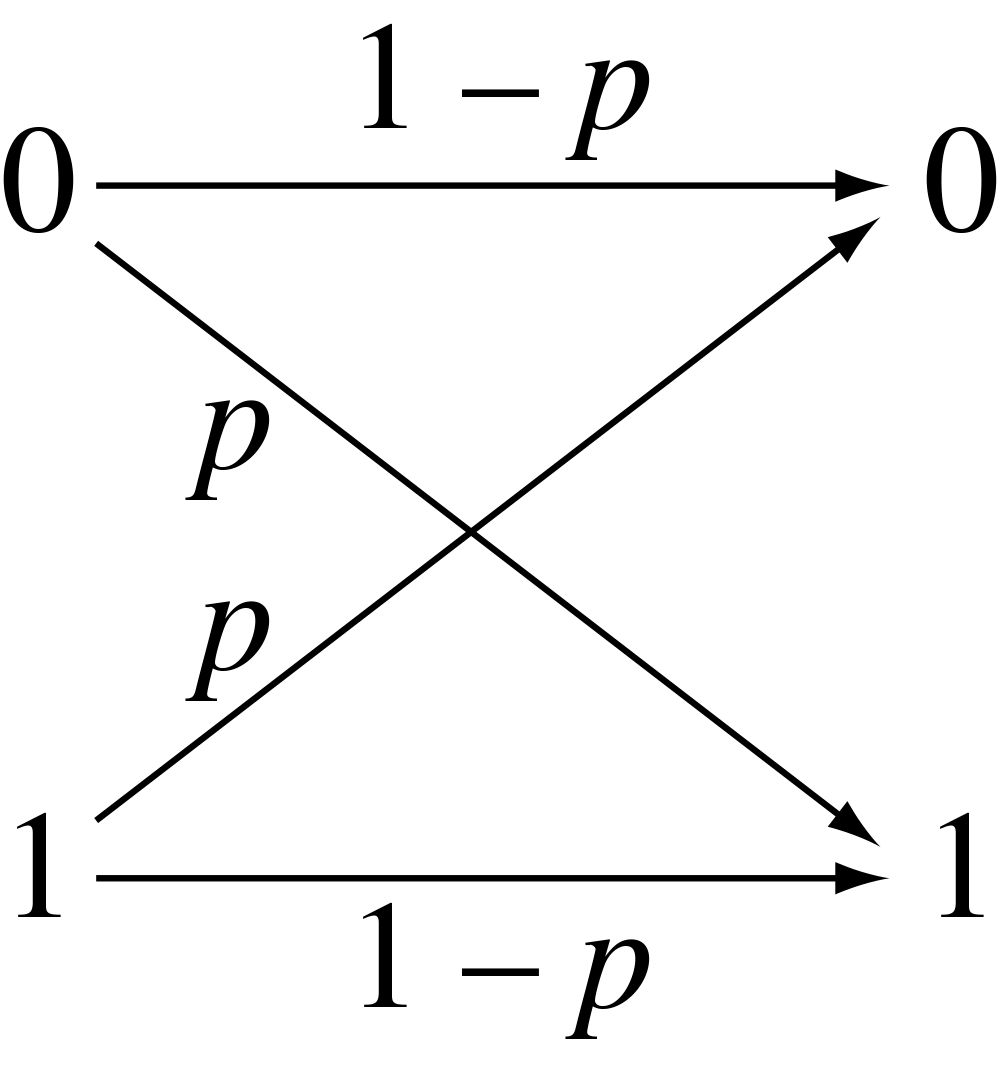
\includegraphics[width=0.3\linewidth]{figures/BSC.png}}
\caption{Το δυαδικό συμμετρικό κανάλι}
\label{fig:BSC channel}
\end{figure}

Αν υποθέσουμε πως το κανάλι είναι \textit{δυαδικό συμμετρικό} (\en{Binary Symmetric Channel - BSC}) κανάλι όπως στο Σχήμα \ref{fig:BSC channel}, η πιθανότητα να συμβεί σφάλμα σε οποιαδήποτε από τις $n$ θέσεις είναι η ίδια - $p$. Συνεπώς υπάρχουν $2^n-1$ διαφορετικά μη-μηδενικά πρότυπα σφάλματος. 

Για την ανίχνευση σφαλμάτων, ο αποκωδικοποιητής υπολογίζει τις παρακάτω $n$-άδες στο $\mathbb{F}_2$:

\begin{equation}
\mathbf{s} = \left(s_0, s_1, \cdots, s_{n-k-1}\right) = \mathbf{r}\cdot\mathbf{H^T}
\label{eq:syndrome formation}
\end{equation}

Το διάνυσμα $\mathbf{s}$ καλείται \textit{σύνδρομο} του $\mathbf{r}$ \cite{ryan2009channel}. Σύμφωνα με την εξίσωση \ref{eq:syndrome formation} και όσα έχουν ήδη αναφερθεί, το ληφθέν διάνυσμα θα είναι κωδικολέξη του $C$ ανν $\mathbf{s}=0$. Σε αντίθετη περίπτωση το ληφθέν διάνυσμα δεν είναι κωδική λέξη περιέχει \textit{σφάλματα μετάδοσης}.

Στην περίπτωση που ισχύει $\mathbf{s}=0$, ο αποκωδικοποιητής θεωρεί το ληφθέν διάνυσμα κωδικολέξη του $C$ χωρίς σφάλματα. Ωστόσο, στην περίπτωση που το $\mathbf{r}$ ανήκει στο κωδικό βιβλίο του $C$ αλλά διαφέρει από την κωδική λέξη που στάλθηκε $\mathbf{v}$, ο αποκωδικοποιητής διαπράττει \textit{σφάλμα αποκωδικοποίησης}. Αυτό συμβαίνει στην περίπτωση που το πρότυπο σφάλματος $\mathbf{e}$ ταυτίζεται με μία κωδική λέξη και καλείται \textit{μη-ανιχνεύσιμο} πρότυπο σφάλματος. Υπάρχουν $2^k-1$ μη-ανιχνεύσιμα πρότυπα σφάλματος \cite{macwilliams1977theory}.

% The decoder (Fig. 1.3) must decide from y which message u or (usually
% simpler) which codeword x was transmitted. Of course it's enough if the
% decoder finds e, for then x = y - e. Now the decoder can never be certain
% what e was. His strategy therefore will be to choose the most likely error
% vector e, given that y was received. Provided the codewords are all equally
% likely, this strategy is optimum in the sense that it minimizes the probability
% of the decoder making a mistake, and is called maximum likelihood decoding.

% Decode y as the nearest codeword x (nearest in Hamming distance), i.e.:
% Pick that error vector e which has least weight.
% This is called nearest neighbor decoding.
% A brute force decoding scheme then is simply to compare y with all 2k
% codewords and pick the closest. This is fine for small codes. But if k is large
% this is impossible! One of the aims of coding theory is to find codes which can
% be decoded by a faster method than this
\subsection{Αποκωδικοποίηση}

Ένας από τους σκοπούς της χρήσης κωδικοποίησης είναι η αύξηση της Ευκλείδιας απόστασης μεταξύ των μεταδιδόμενων σημάτων και κατά συνέπεια, η μείωση της πιθανότητας σφάλματος για δεδομένη ισχύ εκπομπής. Ισοδύναμα, απαιτείται η απόσταση \en{Hamming} μεταξύ των κωδικών λέξεων να είναι η μεγαλύτερη δυνατή. Καθώς ο υπολογισμός της απόστασης \en{Hamming} μεταξύ κάθε κωδικολέξης είναι πρακτικά αδύνατη διαδικασία, η σύγκριση της επίδοσης κωδίκων γίνεται με βάση την ελάχιστη απόσταση $d_{min}$ (ή με βάση το ελάχιστο βάρος $w_{min}$). Συνεπάγεται πως κώδικες με μεγαλύτερη $d_{min}$ έχουν συνήθως καλύτερες επιδόσεις \cite{proakis1994communication}.

Αν θεωρηθεί ο $C(n,k)$ γραμμικός \en{block} κώδικος με πίνακα ελέγχου ισοτιμίας $\mathbf{H}$, ελάχιστη απόσταση $d_{min}(C)$ και το ληφθέν διάνυσμα στο δέκτη,$\mathbf{r}$. Επιγραμματικά αναφέρεται πως, για αποκωδικοποίηση \textit{μέγιστης πιθανοφάνειας} (\en{maximum-likelihood decoding - MLD}), κατά την οποία η απόφαση για τη μεταδιδόμενη κωδικολέξη λαμβάνεται με βάση τη μεγιστοποίηση της υπο-συνθήκη πιθανότητας $P(\mathbf{r}|\mathbf{v})$. Για το κανάλι \en{BSC} του Σχήματος \ref{fig:BSC channel}, αυτό ισοδυναμεί με τον υπολογισμό της απόστασης μεταξύ του $\mathbf{r}$ και κάθε κωδικής λέξης $\mathbf{v}$ και την επιλογή της κωδικής λέξης που ελαχιστοποιεί την απόσταση αυτή. Αυτός ο τρόπος αποκωδικοποίησης ονομάζεται \textit{κοντινότερου γείτονα} (\en{nearest-neighbor}) και αποτελεί αποκωδικοποίηση πλήρους \textit{διόρθωσης σφαλμάτων} (\en{complete error-correction}).

Η συγκεκριμένη μέθοδος αποκωδικοποίησης απαιτεί $2^k$ υπολογισμούς της απόστασης \en{Hamming}. Συνεπώς είναι αδύνατον να υλοποιηθεί πρακτικά. Στη συνέχεια θα δειχθούν μέθοδοι που χαρακτηρίζονται ως μη-πλήρους διόρθωσης σφαλμάτων, για να πετύχουν καλές επιδόσεις και ραγδαία μείωση της πολυπλοκότητας \cite{ryan2009channel}.

\subsection{Πολυπλοκότητα}

Τέλος, αναφορικά με την πολυπλοκότητα, αναφέρεται πως ο ορισμός της έννοιας της πολυπλοκότητας προσεγγίζεται δύσκολα. Ήδη από τη αναπαράσταση ενός γραμμικού \en{block} κώδικα, φαίνεται πως η πολυπλοκότητα περιγραφής (το ποσό μνήμης που χρειάζεται για να αποθηκευτεί ενάς κώδικας), είναι το πολύ $\min\langle Rn^2, \left(1-R\right)n^2\rangle$ \en{bits}, όπου $R$ ο ρυθμός του κώδικα. Επίσης όπως αναφέρθηκε ήδη, η κωδικοποίηση (αποτύπωση του μηνύματος πληροφορίας σε κωδική λέξη) οπώς προκύπτει από την εξίσωση \ref{eq:codeword formation}, γίνεται σε τετραγωνικό χρόνο $\mathcal{O}(n^2)$ \cite{richardson2008modern}.

Η πολυπλοκότητα αποκωδικοποίησης \en{MLD} σε ένα κανάλι \en{BSC} έχει αναλυθεί από τον \en{Berlekamp} κ.α. \cite{berlekamp1978inherent}. Αποδεικνύεται πως η \en{MLD} αποκωδικοποίηση είναι \en{NP-complete}, συνεπώς είναι απίθανο για γραμμικούς κώδικες να έχει πολυωνυμική πολυπλοκότητα \cite{bruck1990hardness}.



	\chapter{\selectlanguage{greek}Κώδικες Επανάληψης-Συσσώρευσης \en{(repeat - accumulate, RA)}}
\externaldocument{chapter1.tex}
\externaldocument{chapter2.tex}

Στο κεφάλαιο αυτό, παρουσιάζονται οι κώδικες Επανάληψης-Συσσώρευσης \en{(repeat - accumulate, RA)}, η μελέτη της επίδοσης των οποίων αποτελεί και το αντικείμενο της παρούσας εργασίας.

Οι \en{RA} αποτελούν τους πρώτους κώδικες που βασίζονται σε συσσωρευτές και εφευρέθηκαν από τους \en{D. Divsalar} κ .ά. \cite{divsalar1998coding}. Ενώ έχουν απλή δομή, δακρίνονται από καλές επιδόσεις, κυρίως στην κατεύθυνση της πρακτικής κωδικοποίησης \en{LDPC} κωδίκων των οποίων αποτελούν υποομάδα, με μοναδικό μειονέκτιμα ότι είναι γενικά χαμηλού ρυθμού (1/2 ή χαμηλότερου). Πλέον, χρηιμοποιούνται ήδη σε αρκετά πρότυπα τηλεπικοινωνιών (\en{DVB-S2,  WirelessMAN IEEE802.16}). Διακρίνονται ως μια ειδική κλαση των \textit{σειριακά συσσωρευμένων} κωδίκων (\en{serially concatenated codes - SC}), στους οποίους ο εξωτερικός κώδικας είναι ένας επαναληπτικός κώδικας ρυθμού $1/q$ και ο εσωτερικός είναι ένας συνελικτικός κώδικας γεννήτορα $\frac{1}{1+D}$, ο οποίος δίνει το $mod-2$ άθροισμα του \en{bit} εισόδου με το προηγούμενο \en{bit} εξόδου. Παράγει δηλαδή το άθροισμα όλων των παρελθόντων εισόδων και για το λόγο αυτό καλείται και \textit{συσσωρρευτής} (\en{accumulator}), στοιχείο που δίνει στος \en{RA} το όνομα τους.

\begin{figure}[h]
\center{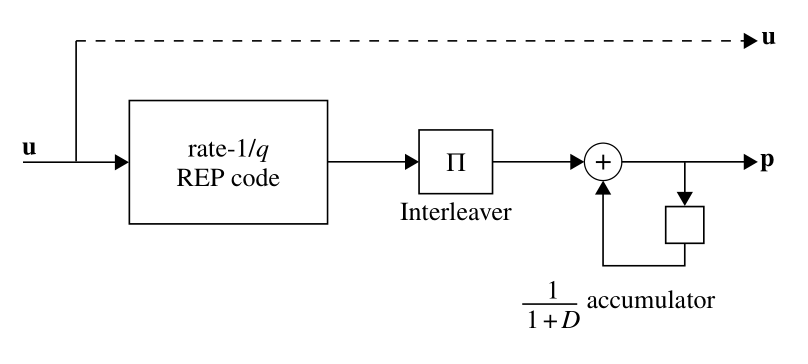
\includegraphics[width=0.65\linewidth]{figures/Ra_scheme.png}}
\caption{\en{Block} διάγραμμα ενός \en{RA} κώδικα}
\label{fig:RA scheme graph}
\end{figure}

Οι \en{RA} που μεταδίδουν τα \en{bits} πληροφορίας και τα \en{bits} ελέγχου ισοτιμίας λέγονται συστηματικοί. Ένα σχηματικό διάγραμα ενός συστηματικόυ \en{RA} κώδικα, φαίνεται στο Σχήμα \ref{fig:RA scheme graph}. Η αποκωδικοποίησή τους μπορεί να αντιμετωπισθεί είτε ως σειριακή \en{turbo}, είτε ως \en{LDPC}, τακτική που είναι και πιο η ευρέως διαδεδομένη \cite{ryan2009channel}.


Στη συνέχεια του κεφαλαίου παρουσιάζονται συνοπτικά οι κώδικες που μπορούν να πλησιάσουν το θεωρητικό όριο χωρητικότητας που επιβάλει το θεώρημα \en{Shannon} (Θεώρημα \ref{theorem:shannon}), διατηρώντας παράλληλα τη δυνατότητα πρακτικής κωδικοποίησης και αποκωδικοποίησης. Αφού γίνει μια σύντομη αναφορά στη σχέση χωρητικότητας και σηματοθορυβικής σχέσης (\en{SNR}), παρουσιάζονται οι τρόποι διαχείρησης των \en{RA}, είτε ως \en{turbo}, είτε ως \en{LDPC}. Κατόπιν αφού αναλυθεί ο τρόπος κωδικοποίησης των \en{LDPC} (ως τον πιο συχνά χρησιμοποιούμενο τρόπο αντιμετώπισης των \en{RA}), διατυπώνεται πλήρως το \en{coding scheme} των \en{RA}, που δίνει και τη βάση πάνω στην οποία στηρίζεται η προσομοίωση που έγινε και θα αναλυθεί στο Κεφάλαιο 4.

\section{Κώδικες που πλησιάζουν τη χωρητικότητα}

Μέχρι και πολύ πρόσφατα, οι κώδικες που μπορούσαν να λειτουργήσουν κοντά στο θεωρητικό όριο χωρητικότητας που προέβλεπε το θεώρημα \en{Shannon}, ήταν κυρίως μεγάλοι σε μήκος, μη πρακτικοί κώδικες. Με την ανακάλυψη των \en{turbo} κωδίκων και την επανανακάλυψη των \en{LDPC} τη δεκαετία του '90, έγινε δυνατό να αποδειχθεί η ικανότητα λειτουργίας τους κοντά στη χωρητικότητα, με πρακτικά υλοποιήσιμους κωδικοποιητές-αποκωδικοποιητές σε σχετικά μεσαία \en{bit error rates (BERs)}, μέσω του καναλιού \en{AWGN}. 

Παρ'όλο που η θεωρητική επίτευξη του ορίου χωρητικότητας αφορά κώδικες με άπειρο μήκος, στην πράξη αρκεί το μήκος του κώδικα να είναι αρκετά μεγάλο (π.χ. $n\geq5000$) ώστε να υπάρχει ικανοποιητική απόδοση κοντά στο θεωριτικό όριο. Η σχεδίαση τέτοιων κωδίκων χαρακτηρίζεται από 2 βασικά στοιχεία:
\begin{itemize}
\item Χρήση κωδίκων αποτελούμενων από απλά μέρη, συνενωμένα με τρόπο που να παράγεται μια ψευδο-τυχαία κατανομή βαρών και,
\item Χρήση μη-βέλτιστων επαναληπτικών αλγορίθμων αποκωδικοποίησης με συνεχή ανταλλαγή \en{soft} πληροφορίας, των οποίων η πολυπλοκότητα αυξάνει γραμμικά με την αύξηση του μήκους κώδικα.
\end{itemize}

Μπορεί επίσης να δοθεί και ο παρακάτω ορισμός των κωδίκων που πλησιάζουν τη χωρητικότητα:
\begin{definition}\en{Capacity-approaching} κώδικες

Έστω μια αλληλουχία από δυαδικούς γραμμικούς κώδικες $\left( C_m \right)$, ρυθμού $R_m$ και για κάθε κώδικα, οι κωδικές λέξεις μεταδίδονται ισοπίθανα μέσω ενός καναλιού με χωρητικότητα $C$. Η αλληλουχία επιτυγχάνει κλάσμα $1-\epsilon$ της χωρητικότητας του καναλιού αν $\lim_{m\to \infty}R_m\geq\left(1-\epsilon\right)\cdot C$ και υπάρχει αλγόριθμος αποκωδικοποίησης για τον οποίο η πιθανότητα εσφαλμένου \en{bit} του κώδικα $C_m$ τείνει στο μηδέν, όταν $m\to \infty$ \cite{pfister2005capacity}.
\label{def:capacity approaching codes}
\end{definition}

Οι \en{capacity-approaching} κώδικες χωρίζονται σε δύο μεγάλες υποκατηγορίες: τους \en{turbo} ή \en{turbo-like} κώδικες, οι οποίοι διακρίνονται από συνελικτικούς \en{component codes} χαμηλής πολύπλοκότητας και κάνουν χρήση του επαναληπτικού αποκωδικοποιητή αθροίσματος γινομένου (\en{sum-product decoder}) και τους κώδικες Πίνακα Ισοτιμίας Χαμηλής Πυκνότητας (\en{Low Density Parity Check - LDPC}).

\begin{figure}[h]
\center{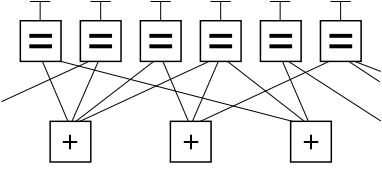
\includegraphics[width=0.65\linewidth]{figures/LDPC_factor_graph.png}}
\caption{Μέρος του γραφήματος παραγόντων ενός \en{LDPC} κώδικα}
\label{fig:LDPC factor graph}
\end{figure}


Οι \en{LDPC} κώδικες, κατά κύριο λόγο χρησιμοποιούν \en{component codes} μονού ελέγχου ισοτιμίας και επαναληπτική ανταλλαγή μυνημάτων (με τη μορφή πιθανοτήτων) για την αποκωδικοποίηση, που βασίζεται σε διμερή γραφήματα. Και οι δύο κατηγορίες που περιγράφηκαν, διακρίνονται από κοινά στοιχεία. Kάνοντας χρήση γενικής αναπαράστασης με γραφήματα παραγόντων (\en{factor-graph representation}) οι \en{turbo} κώδικες θεωρούνται πλέον μια γενίκευση των \en{LDPC}. Επίσης πλέον, όλοι οι \en{capacity-approaching} κώδικες μπορούν να ομαδοποιηθούν ως οικογένεια Κωδίκων σε Γραφήματα (\en{Codes on Graphs}) \cite{ryan2009channel}, \cite{johnson2009iterative}, \cite{codes2009guest}.

\subsection{Η χωρητικότητα ως \en{SNR}}

Σε αυτό το σημείο θα γίνει μια σύντομη αναφορά στη σχέση που συνδέει τη χωρητικότητα ενός καναλιού με τη σηματοθορυβική σχέση \en{SNR} που το χαρακτηρίζει.

Έστω τηλεπικοινωνιακό σύστημα, με ζωνοπερατό κανάλι, εύρους ζώνης $W$, που εισάγει \en{AWGN} θόρυβο, με φασματική πυκνότητα ισχύος $N_0/2$. Η χωρητικότητα καναλιού αποδεικνύεται ότι μπορεί να οριστεί από την παρακάτω εξίσωση (Θεώρημα \en{Shannon - Hartley}):

\begin{equation}
C=W\cdot log_2(1+ \frac{S}{N})
\label{eq:capacity}
\end{equation}
όπου, $S$ η λαμβανόμενη ισχύς του μεταδιδόμενου σήματος στο δέκτη, $N$ η ισχύς θορύβου και $W$ το εύρος ζώνης του καναλιού. Από την εξίσωση \ref{eq:capacity} καθώς και το Σχήμα \ref{fig:Channel capacity}, διακρίνονται οι δύο οριακές περιπτώσεις για την τιμή της χωρητικότητας σε σχέση με το \en{SNR}.
\begin{itemize}
\item Για μεγάλα \en{SNR} ($SNR \gg 0$) η χωρητικότητα εκφράζεται από τη σχέση $C\approx W\log_{2}{\frac{S}{N}}$, είναι δηλαδή λογαριθμικής δύναμης και σχεδόν γραμμική σε σχέση με το εύρος ζώνης. Η περιοχή αυτή καλείται \textit{\en{bandwidth-limited regime}}
\item Για μικρά \en{SNR} ($SNR \ll 0$) η χωρητικότητα εκφράζεται από τη σχέση $C\approx W\cdot\frac{S}{N}\log_{2}{e}$, είναι δηλαδή γραμμικής δύναμης αλλά δεν επηρεάζεται από το εύρος ζώνης. Η περιοχή αυτή καλείται \textit{\en{power-limited regime}}
\end{itemize}


\begin{figure}[h]
\center{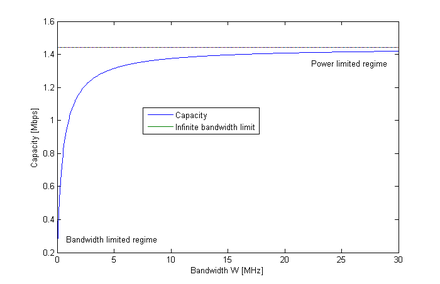
\includegraphics[width=0.55\linewidth]{figures/Channel_capacity.png}}
\caption{Χωρητικότητα ζωνοπερατού καναλιού ως προς το εύρος ζώνης}
\label{fig:Channel capacity}
\end{figure}

Η ισχύς του θορύβου δίνεται από τη σχέση:

\begin{equation}
N = \int_{-W}^{W}\frac{N_0}{2}\,df=N_0\cdot{W}.
\label{eq:Noise}
\end{equation}
,ενώ η συματοθορυβική σχέση του συστήματος (\en{signal-to-noise ratio - SNR}) ορίζεται ως:

\begin{equation}
SNR=\frac{S}{N}
\label{eq:SNR}
\end{equation}

Από τις \ref{eq:capacity} και \ref{eq:SNR} και κανονικοποιώντας ως προς το εύρος ζώνης $W$, προκύπτει:

\begin{equation}
C=log_2(1+SNR)
\label{eq:capacity vs SNR}
\end{equation}
σχέση που αποτελεί και το άνω όριο του ρυθμού για αξιόπιστη επικοινωνία σύμφωνα με το Θεώρημα \ref{theorem:shannon} (Θεώρημα Κωδικοποίησης Ενθόρυβου Καναλιού).

\section{\en{RA} ως \en{turbo}}

Σε αυτή την παράγραφο, θα γίνει μια σύντομη αναφορά στους κώδικες \en{turbo}, της ιδιότητες που χαρακτηρίζουν την αποκωδικοποίησή τους, καθώς και την δυνατότητα των \en{RA} να χαρακτηριστούν ως τέτοιοι.

\subsection{Κώδικες \en{turbo}}

Οι κώδικες \en{turbo} ανακαλύφθηκαν από τους \en{Berrou, Glavieux} και \en{Thitimajshima} \cite{berrou1993near} το 1993 και αποτέλεσαν ριζοσπαστική προσέγγιση της κωδικοποίησης για διόρθωση σφαλμάτων. Αποτελούνται από τον παράλληλο συνδυασμό δύο συνελικτικών κωδίκων, οι οποίοι κατά την αποκωδικοποίηση διαμοιράζουν πληροφορία μεταξύ των αντίστοιχων αποκωδικοποιητών. Αναφέρεται πως ο κωδικοποιητής χρησιμοποιεί συνελικτικούς κώδικες \cite{hagenauer1996iterative}, ενώ ο αποκωδικοποιητής χρησιμοποιεί \en{BCJR} κώδικες \cite{abrantes2004bcjr}.

\begin{figure}[h]
    \centering
    \begin{minipage}{0.45\textwidth}
        \centering
        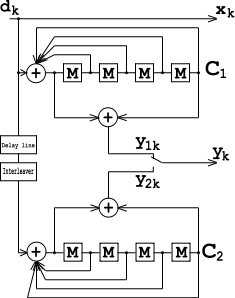
\includegraphics[width=0.9\textwidth]{figures/Turbo_encoder.png}
        \caption{Κωδικοποιητής \en{turbo}}
    \end{minipage}\hfill
    \begin{minipage}{0.45\textwidth}
        \centering
        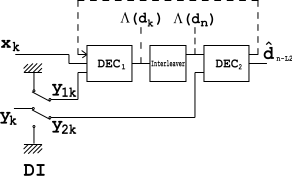
\includegraphics[width=0.9\textwidth]{figures/Turbo_decoder.png}
        \caption{Αποκωδικοποιητής \en{turbo}}
    \end{minipage}
\end{figure}

Ο κωδικοποιητής \en{turbo} περιέχει έναν \textit{παρεμβολέα} (\en{interleaver}), ο ρόλος του οποίου είναι να μεταθέτει κωδικές λέξεις μικρού βάρους από τον ένα κωδικοποιητή σε κωδικές λέξεις μεγάλου βάρους στον άλλο, με διάφορους τρόπους. Επιγραμματικά αναφέρεται ο \en{\textit{row-column} interleaver}, o \en{\textit{helical}} kai o \en{\textit{odd-even} interleaver}.

Η αποκωδικοποίηση απαιτέι τον υπολογισμό πιθανοτικών μετρικών \en{log-likelihood ratios (LLRs)} και την πρόβλεψη για το μεταδιδόμενο σύμβολο $\mathbf{y_k}$, με βάση την εγγύτητά του στο 0 ή στο 1, καθώς και χρησιμοποιώντας \en{Hard-Desicion} αποκωδικοποίηση \cite{berrou1993near}.

\subsection{\en{RA} ως \en{turbo}}

Το συνολικό \en{coding scheme} των \en{RA} που προσομοιώθηκε θα αναλυθεί στη συνέχεια του κεφαλαίου. Ωστόσο, η αποκωδικοποίηση τους μπορεί να βασιστεί στην \en{turbo} αποκωδικοποίηση των \en{SC}, όπου, όπως αναφέρθηκε ήδη, ο εξωτερικός κώδικας είναι \en{repetition} και ο εσωτερικός είναι ο \en{accumulator}. Για τους συστηματικούς \en{RA} κώδικες που περιέχουν συνδυαστή, ο εσωτερικός κώδικας είναι συνδυαστικός αποκωδικοποιητής συνδυαστή-συσσωρευτή (\en{accumulator-combiner - AC}) και ο \en{REP} αποκωδικοποιητής έχει ως είσοδο τα \en{LLRs} από το κανάλι \cite{johnson2009iterative}.

\begin{figure}[h]
\center{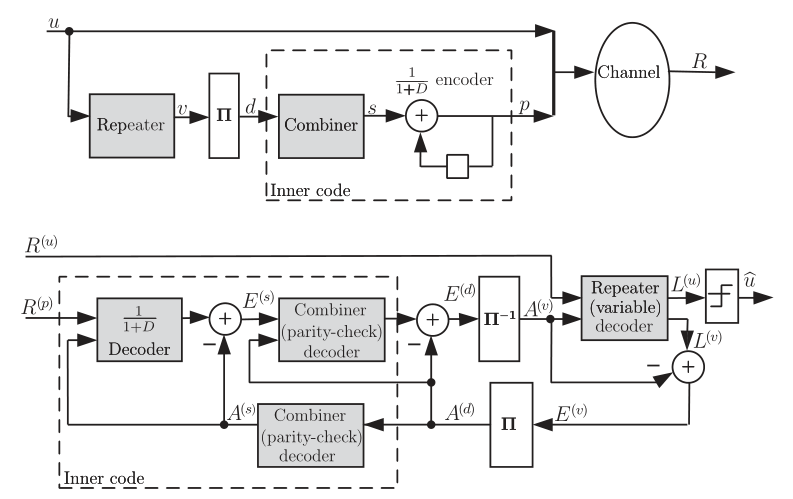
\includegraphics[width=0.85\linewidth]{figures/systematic_RA.png}}
\caption{Κωδικοποιητής / \en{turbo} αποκωδικοποιητής συστηματικού \en{RA}}
\label{fig:enc/turbo dec of systematic RA}
\end{figure}

Στο Σχήμα \ref{fig:enc/turbo dec of systematic RA}, φαίνεται η κωδικοποίηση και αποκωδικοποίηση \en{turbo} ενός \en{RA} κώδικα, βάση της \textit{αρχής \en{turbo}} (\en{turbo principle}) \cite{hagenauer2003turbo}. Σε κάθε επανάληψη της αποκωδικοποίησης, ο \en{REP} αποκωδικοποιητής λαμβάνει \en{LLRs} από το κανάλι αναφορικά με τα \en{bits} πληροφορίας και στις επόμενες επαναλήψεις, τα \en{a-priori LLRs} εξωγενούς πληροφορίας από τον \en{AC} αποκωδικοποιητή, από τις προηγούμενες επαναλήψεις.

Στο επόμενο βήμα ο \en{REP} αποκωδικοποιητής υπολογίζει τα \en{LLRs} εξόδου. Η εξωγενής πληροφορία από τον \en{REP} αποκωδικοποιητή, παρεμβάλλεται από τον \en{interleaver} για την παραγωγή \en{a-priori LLRs} στον \en{AC} αποκωδικοποιητή. Στην τελική επανάληψη, υπολογίζεται η κωδική λέξη από τα \en{a posteriori LLRs} για τα \en{bits} πληροφορίας από το κανάλι και τα \en{a-priori LLRs} από τον \en{AC} αποκωδικοποιητή για τα κωδικά \en{bits}. Ο αλγόριθμος τελειώνει μετά από ένα προκαθορισμένο αριθμό $I_{max}$ επαναλήψεων. Σε περίπτωση μη-συστηματικού \en{RA} τα υπολογιζόμενα \en{LLRs} για τα \en{bits} πληροφορίας είναι μηδέν \cite{johnson2009iterative}.


\section{\en{RA} ως \en{LDPC}}

Οι κώδικες \en{LDPC} παρουσιάστηκαν για πρώτη φορά το 1962 από τον \en{R. G. Gallager} στη διδακτορική του διατριβή \cite{gallager1962low} και αποτελούν κώδικες διόρθωσης σφαλμάτων που ορίζονται από αραιό πίνακα ελέγχου ισοτιμίας. Παρά το ότι αποτελούν \en{capacity-approaching} κώδικες εγκαταλείφθηκαν για περίπου 30 χρόνια, με εξαίρεση τη δουλειά του \en{Tanner} \cite{tanner1981recursive} που εισήγε και τη γραφική αναπαράσταση τους, μέσω του γραφήματος \en{Tanner}, λόγω περιορισμών στην τεχνική τους υλοποίηση και επανακαλύφθηκαν το 1996 από τους \en{Mackay} κ.α. \cite{mackay1996near}. Tο κύριο χαρακτηριστικό τους, η χαμηλή πυκνότητα του πίνακα $\mathbf{H}$, είναι και αυτό που κάνει τους \en{LDPC} να επιδέχονται διάφορους αλγόριθμους επαναληπτικής αποκωδικοποίησης (\en{iterative decoding}). Παρ’ότι οι αλγόριθμοι επαναληπτικής αποκωδικοποίησης έχουν μη-βέλτιστη απόδοση, μπορούν να έχουν απόδοση που χαρακτηρίζεται “σχεδόν” βέλτιστη (\en{near-optimal}), σε εφαρμογές/\en{error-rates} ενδιαφέροντος και διακρίνονται από καλύτερες επιδόσεις στη διόρθωση σφαλμάτων σχετικά με τους \en{turbo}.

Κάθε γραμμικός κώδικας έχει αναπαράσταση μέσω πίνακα ελέγχου-ισοτιμίας, ωστόσο για να αποτελεί \enquote*{αραιή} η αναπαράσταση πρέπει να πλοιρούνται ορισμένα κριτήρια. Ένας $n\times m$ πίνακας καλείται αραιός αν το ποσό από άσσους (1) στις γραμμές και στις στήλες του, το βάρος γραμμών ($w_r$) και στηλών ($w_c$) αντίστοιχα, είναι πολύ μικρότερο από τις διαστάσεις του ($w_r\ll m$, $w_c\ll n$). Πρακτικά, θεωρείται πως αν το $1\%$ των στοιχείων του πίνακα είναι άσσοι, τότε εί77ναι αραιός. Αν το βάρος γραμμών και στηλών είναι σταθερό ο κώδικας \en{LDPC} λέγεται ομαλός, ενώ σε αντίθετη περίπτωση λέγεται ανώμαλος \cite{ta2013tutorial}.

Γενικά, εκτός από την απαίτηση να είναι ο πίνακας $\mathbf{H}$ αραιός, οι \en{LDPC} δε διαφέρουν από τους \en{block} κώδικες. Ωστόσο, η εύρεση ενός αραιού πίνακα ελέγχου ισοτιμίας για ένα δεδομένο \en{block} κώδικα αποτελεί δύσκολη διαδικασία και αντίθετα της κατασκευής των \en{LDPC} προηγείται η κατασκευή του πίνακα $\mathbf{H}$ και ακολουθεί η σχεδίαση του κωδικοποιητή. Λόγω αυτού οι \en{LDPC} αποκωδικοποιούνται επαναληπτικά, κάνοντας χρήση γραφικής αναπαράστασης του πίνακα ελέγχου ισοτιμίας και σχεδιάζονται με γνώμονα τις ιδιότητές του.

Έχει διαπιστωθεί πως και οι \en{RA} και οι  \en{LDPC} ενέχουν πλεονέκτημα σε σχέση με τους \en{turbo} κώδικες, καθώς προσφέρουν μια πιο ευέλικτη δομή, κάτι που με τη σειρά του προσφέρει περισσότερους βαθμους ελευθερίας στην επιλογή των παραμέτρων για δεδομένο κριτήριο σχεδίασης \cite{johnson2009iterative}.

\subsection{Κωδικοποίηση \en{LDPC}}

Όπως αναφέρθηκε στο Κεφάλαιο 2, οι γραμμικοί \en{block} κώδικες αποτυπώνουν το μήνυμα πληροφορίας $\mathbf{u}$ στην κωδική λέξη $\mathbf{v}$ κάνοντας χρήση της εξίσωσης \ref{eq:check equation}, για δοσμένο γεννήτορα πίνακα $\mathbf{G}$. Γενικά, όπως έχει επίσης αναφερθεί και στο Κεφάλαιο 2, ο πίνακας $\mathbf{G}$ ενός κώδικα δίνεται από το \en{null-space} του -αραιού για τους \en{LDPC}- πίνακα $\mathbf{H}$. Συνεπώς είναι απίθανο να είναι και ο ίδιος αραιός, κάτι που θα οδηγούσε σε γραμμικό χρόνο κωδικοποίησης (ως προς το μήκος του κώδικα). Προκύπτει επομένως πως, η κωδικοποίηση ενός \en{LDPC} με βάση την εξίσωση \ref{eq:check equation} γίνεται σε τετραγωνικό χρόνο ως προς το μήκος κώδικα. Σημειώνεται πως έχουν γίνει διάφορες προσπάθειες προς την κατεύθυνση της μείωσης του χρόνου αυτού \cite{ta2013tutorial}. Ωστόσο, οι κώδικες \en{LDPC} κατασκευάζονται με γνώμονα τον πίνακα ελέγχου ισοτιμίας $\mathbf{H}$. Συνεπώς, η κωδικοποίησή τους, ακολουθεί διαφορετική πορεία. 

Αρχικά, το μήνυμα πληροφορίας αποτυπώνεται στην κωδική λέξη ως εξής:

\begin{equation}
\begin{split}
\mathbf{v} &= \mathbf{G}^T\mathbf{u} \\
\Rightarrow \mathbf{0} &= \mathbf{H}\mathbf{G}^T\mathbf{u} \\
\Rightarrow \mathbf{0} &= \mathbf{H}\mathbf{G}^T
\end{split}
\label{eq:LDPC encoding}
\end{equation}

Θεωρώντας συστηματική κωδικοποίηση, και υπενθυμίζοντας πως ο συστηματικός γεννήτορας πίνακας μπορεί να γραφεί ως $\mathbf{G} = \left[\mathbf{P}\;\;\mathbf{I_k}\right]$, προκύπτει πως

\begin{equation}
\begin{split}
\mathbf{H}\mathbf{G}^T &= \mathbf{H_1}\mathbf{I_k} + \mathbf{H_2}\mathbf{P}^T \\
\Rightarrow \mathbf{P}^T &= \mathbf{H_2}^{-1}\mathbf{H_1}
\end{split}
\label{eq:parity part of LDPC}
\end{equation}
και λαμβάνοντας υπ'όψη την εξίσωση \ref{eq:LDPC encoding} προκύπτει η κωδική λέξη (σχηματικά στο Σχήμα \ref{fig:LDPC codeword formation})

\begin{equation}
\mathbf{v} = \mathbf{G}^T\mathbf{u} = \left[\mathbf{P}\;\;\mathbf{I_k}\right]^T\mathbf{u} = \left[\mathbf{u}\;\;\mathbf{H_2}^{-1}\mathbf{H_1}\mathbf{u}\right]^T
\label{eq:LDPC codeword formation}
\end{equation}

\begin{figure}[h]
\center{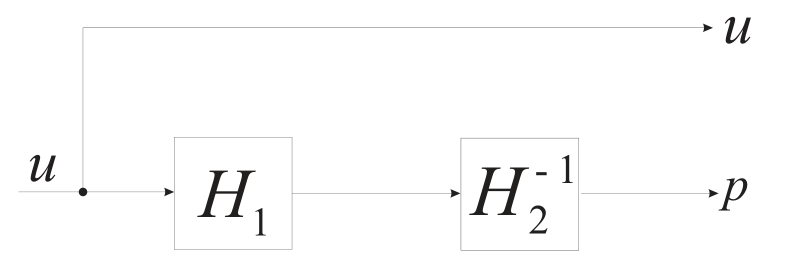
\includegraphics[width=0.75\linewidth]{figures/LDPC_encoding.png}}
\caption{Διαμόρφωση συστηματικής κωδικής λέξης \en{LDPC} κώδικα}
\label{fig:LDPC codeword formation}
\end{figure}

\subsection{Κωδικοποίηση \en{RA}}

Το \en{block} διάγραμμα διαμόρφωσης της κωδικής λέξης ενός \en{RA} κώδικα, δόθηκε ήδη στο Σχήμα \ref{fig:RA scheme graph}. Η κωδικοποίηση \en{RA} ακολουθεί την συστηματική \en{LDPC}. Τα \en{bits} πληροφορίας αντιγράφονται $q$ φορές, περνούν από τον παρεμβολέα, ομαδοποιούνται μέσω $mod-2$ πρόσθεσης σε \en{block} μήκους $a$ και τέλος περνούν από ένα συνελικτικό κωδικοποιητή μνήμης -1.

Συγκεκριμένα, το μήνυμα πληροφορίας μήκους $k$, $\mathbf{u}=\left(u_0,u_1,\cdots,u_{k-1}\right)$, μετά την έξοδο από τον επαναληπτικό κωδικοποιητή, έχει τη μορφή:

\begin{equation}
\begin{split}
\mathbf{c} &= \left[c_1, c_2, \cdots, c_{qk} \right] \\
&= (\underbrace{u_1,u_1,\cdots,u_1}_q, \; \underbrace{u_2,u_2,\cdots,u_2,}_q, \; \cdots, \; \underbrace{u_{qk},u_{qk},\cdots,u_{qk}}_q)
\end{split}
\end{equation}
, όπου $c_i=u_{f(i)}$ με $f(i)=\lceil i/q \rceil$ και $\lceil x \rceil$ το άνω κατώφλι του $x$.

Κατόπιν, κατα την έξοδο από τον παρεμβολέα $\Pi=[\pi_1,\pi_2,\cdots,\pi_{qk}]$, διαμορφώνεται μια μετάθεση της ακολουθίας $\mathbf{c}$ ως εξής:

\begin{equation*}
\mathbf{d} = \left[d_1, d_2, \cdots, d_{qk} \right] = [c_{\pi_1}, c_{\pi_2}, \cdots, c_{\pi_{qk}}]
\end{equation*}

Ο συνδυαστής λαμβάνει την έξοδο του παρεμβολέα και προσθέτει ($mod-2$) και ομαδοποιεί τα \en{bits} σε \en{block} μήκους $a$. Τα \en{bits} της ακολουθίας εξόδου του συνδυαστη $\mathbf{s}$, δίνονται από την εξίσωση:

\begin{equation}
s_i=d_{a(i-1)+1}\oplus d_{a(i-1)+2} \oplus \cdots \oplus d_{ai}, \;\;\; i=1,2,\cdots,m\;\;m=kq/a
\label{eq:combiner equation}
\end{equation}

Στην έξοδο του συσσωρευτή, τα \en{parity bits} θα δίνονται από την εξίσωση:

\begin{equation}
p_i=p_{i-1}\oplus s_i\;\;\; i=1,2,\cdots,m
\label{eq:accumulator equation}
\end{equation}

Από την εξίσωση \ref{eq:accumulator equation}, προκύπτει πως η κωδική λέξη του συστηματικού \en{RA} κώδικα, έχει τη μορφή $\mathbf{v}=[u_1, u_2,\cdots,u_k,p_1,p_2,\cdots,p_m]$, οπότε το μήκος του κώδικα προκύπτει $n=k(1+q/a)$ και ο ρυθμός $R=a/(a+q)$ \cite{johnson2009iterative}.

\subsection{Αποκωδικοποίηση \en{RA}}

Αναφέρθηκε ήδη η δυνατότητα των \en{RA} κωδίκων για \en{turbo} αποκωδικοποίηση. Ωστόσο, στο πλαίσιο της συγκεκριμένης εργασίας, μελετάται η δυνατότητα για αποκωδικοποίηση ως \en{LDPC}, χρησιμοποιώντας τον αλγόριθμο \en{\textit{Sum-Product}}.

Ο αλγόριθμος παρουσιάστηκε από τον \en{Gallager} μαζί με τους κώδικες \en{LDPC}. Χαρακτηρίζεται από \en{near-optimal} επίδοση αποκωδικοποίησης καθώς και από καθολικότητα για τα διάφορα κανάλια χωρίς μνήμη (\en{BEC, BSC, BI-AWGN}, κ.λ.π.), συνεπώς η ανάπτυξή του είναι γενική. Το κριτήριο βέλτιστης ανάπτυξης του αλγορίθμου, είναι ο υπολογισμός της μέγιστης εκ των υστέρων (\en{maximum a posteriori - MAP}) πιθανότητα. Υπολογίζεται δηλαδή η (εκ των υστέρων) πιθανότητα για την τιμή κάθε συγκεκριμένου \en{bit} της κωδικής λέξης $\mathbf{v}$, με δεδομένο το ληφθέν διάνυσμα $\mathbf{r}$.

\subsubsection{Ο \en{Sum-Product} αλγόριθμος για \en{LDPC}}

Η αποκωδικοποίηση του κωδικού \en{bit} $v_j$ (χωρίς βλάβη της γενικότητας) απαιτεί τον υπολογισμό της \en{APP} πιθανότητας (για τιμή \en{bit} 1):
\begin{equation*}
\Pr(v_j=1|\mathbf{r})
\end{equation*}
το λόγο \en{APP}
\begin{equation*}
l(v_j|\mathbf{r})\triangleq\frac{\Pr(v_j=0|\mathbf{r})}{\Pr(v_j=1|\mathbf{r})}
\end{equation*}
ή το (σταθερότερο αριθμητικά) λόγο \en{log-APP}, που καλείται επίσης \en{log-likelihood ration (LLR)}:

\begin{equation}
L(v_j|\mathbf{r})\triangleq\log\left(\frac{\Pr(v_j=0|\mathbf{r})}{\Pr(v_j=1|\mathbf{r})}\right)
\label{eq:LLR}
\end{equation}

\begin{figure}[h]
\center{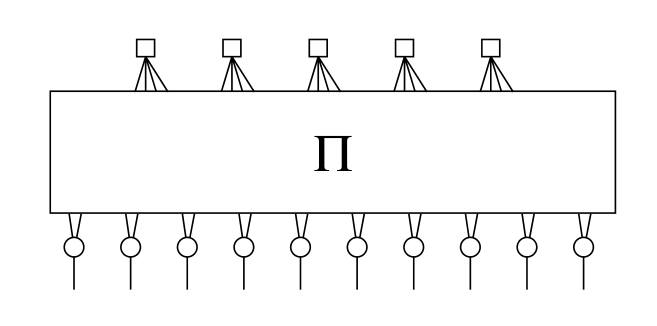
\includegraphics[width=0.6\linewidth]{figures/LDPC_graphical.png}}
\caption{Αναπαράσταση \en{LDPC} ως αλληλουχία από \en{SPC} (κάτω) και \en{REP} (επάνω) κώδικες. Με $\Pi$ συμβολίζεται ο παρεμβολέας}
\label{fig:LDPC graphical}
\end{figure}

Ο υπολογισμός της εξίσωσης \ref{eq:LLR} γίνεται εφαρμόζοντας την αρχή \en{turbo} στο γράφημα \en{Tanner}. Με αναφορά το Σχήμα \ref{fig:LDPC graphical}, ο \en{LDPC} μπορεί να θεωρηθεί ως ένα σύνολο από \en{SPC} κώδικες συνδεόμενους μέσω του παρεμβολέα σε ένα σύνολο \en{REP} κωδίκων. Οι \en{SPC} κώδικες (\en{CNs} στο γράφημα \en{Tanner}) θεωρούνται εξωτερικοί κώδικες, συνεπώς δε συνδέονται στο κανάλι.

Τα Σχήματα \ref{fig:VN}, \ref{fig:CN} αναπαριστούν στιγμιότυπα των \en{REP} και \en{SPC} αποκωδικοποιητών (κόμβοι \en{VN} και \en{CN} αντίστοιχα).

\begin{figure}[h]
    \centering
    \begin{minipage}{0.45\textwidth}
        \centering
        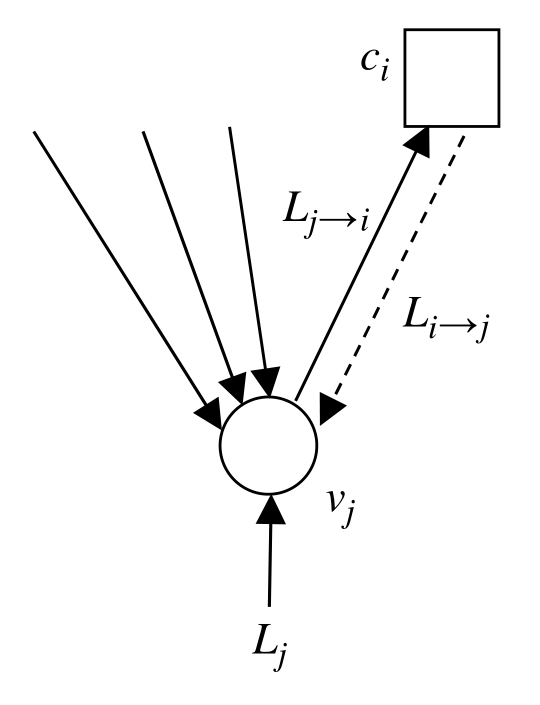
\includegraphics[width=0.9\textwidth]{figures/VN.png}
        \caption{Ο κόμβος \en{VN} $j$ (αποκωδικοποιητής κώδικα \en{REP}) λαμβάνει πληροφορία από τους γειτονικούς \en{CN} (εκτός από τον $i$ $(L_{i\to j})$) και στέλνει στον \en{CN} $i$ την ποσότητα $L_{j\to i}$}
        \label{fig:VN}
    \end{minipage}\hfill
    \begin{minipage}{0.45\textwidth}
        \centering
        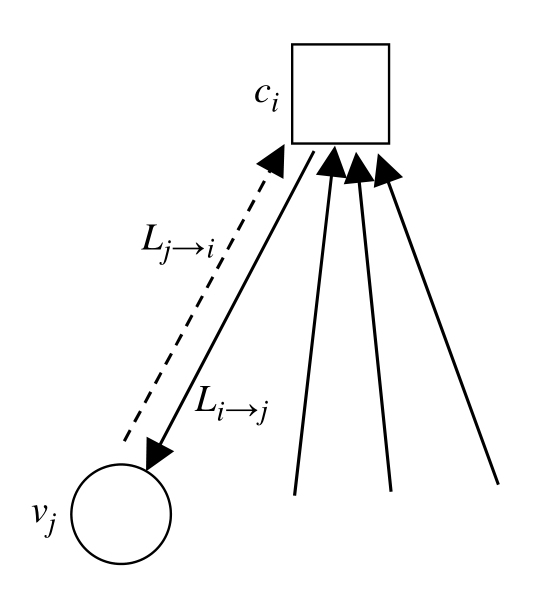
\includegraphics[width=0.9\textwidth]{figures/CN.png}
        \caption{Ο κόμβος \en{CN} $i$ (αποκωδικοποιητής κώδικα \en{SPC}) λαμβάνει πληροφορία από τους γειτονικούς \en{VN} (εκτός από τον $j$ $(L_{j\to i})$) και στέλνει στον \en{VN} $j$ την ποσότητα $L_{i\to j}$}
        \label{fig:CN}
    \end{minipage}
\end{figure}

Οι αποκωδικοποιητές (κόμβοι) \en{VN} και \en{CN} λειτουργούν συνεργατικά για τον υπολογισμό της εκτίμησης $L(v_j|\mathbf{r}),\;\;j=0,1,\cdots,n-1$, επαναληπτικά. Κατά τη λειτουργία τους, υιοθετείται το \en{\textit{flooding schedule}}, σύμφωνα με το οποίο ξεκινώντας από τους \en{VN}, οι \en{VN} (\en{CN}) επεξεργάζονται την είσοδο και υπολογίζουν \textit{εξωγενή πληροφορία} την οποία στέλνουν στους γειτονικούς \en{CN} (\en{VN}). Η διαδικασία ολοκληρώνεται μετά από ένα προκαθορισμένο αριθμό επαναλήψεων ή αφού εκπληρωθεί ένα κριτήριο τερματισμού και υπολογίζεται η πιθανότητα $L(v_j|\mathbf{r})$, μέσω της οποίας λαμβάνεται απόφαση για την τιμή του \en{bit} $v_j$. Η υλοποίηση του \en{SPA} βασίζεται επίσης στη \textit{υπόθεση ανεξαρτησίας}: οι ληφθείσες ποσότητες \en{LLR} σε κάθε κόμβο από τους γειτονικούς, είναι μεταξύ τους ανεξάρτητες.

Θα χρειαστεί να αναφερθούν επίσης οι εσωτερικές διαδικασίες και υπολογισμοί, που λαμβάνουν χώρα στους κόμβους \en{VN} και \en{CN} αντίστοιχα, για τον υπολογισμό της μετρικής \en{LLR} που ανταλλάσσεται μεταξύ γειτονικών κόμβων. Θεωρείται πως αντί για \en{MAP} αποκωδικοποιητές, οι \en{VN} και \en{CN} λειτουργούν σαν \en{APP} επεξεργαστές για \en{REP} και \en{SPC} κώδικες αντίστοιχα, σε κάθε επανάληψη του αλγορίθμου.

Η εξωγενής πληροφορία που στέλνεται από τον \en{VN} $j$ στον \en{CN} $i$ δίνεται από τη εξίσωση:

\begin{equation}
L_{j\to i} = L_j + \sum_{i'\in N(j)-\lbrace i\rbrace} L_{i'\to j}
\label{eq:CN update}
\end{equation}
, όπου η ποσότητα $L_j$ δίνεται από την εξίσωση \ref{eq:LLR}. Αντίστοιχα, η εξωγενής πληροφορία που στέλνεται από τον \en{CN} $i$ στον \en{VN} $j$, δίνεται από την παρακάτω εξίσωση:

\begin{equation}
L_{i\to j} = 2\tanh^{-1} \left( \prod_{j'\in N(i)-\lbrace j\rbrace} \tanh \left( \frac{1}{2}L_{j'\to i} \right)\right)
\label{eq:VN update}
\end{equation}
Στο τέλος των επαναλήψεων, ο \en{VN} $j$ παράγει μια πρόβλεψη με βάση την ποσότητα

\begin{equation}
L_{j}^{total} = L_j + \sum_{i\in N(j)} L_{i\to j}
\label{eq:LLR total}
\end{equation}

Η πληροφορία $L_{j\to i}$ που ανταλάσσεται μεταξύ των \en{VN} $j$ και \en{CN} $i$, απότελεί τη βέλτιστη (εξωγενή) εκτίμηση της τιμής του $v_j$ (πρόσημο του $L_{j\to i}$) και το επίπεδο εμπιστοσύνης της τιμής (πλάτος του $L_{j\to i}$), βασισμένη στο \en{REP constraint} για τον αντίστοιχο κόμβο. Αντίστοιχα, η εκτίμηση του \en{CN} $i$ βασίζεται στο \en{SPC constraint}. Τέλος αναφέρεται πως για την αρχικοποίηση, χρησιμοποιείται η εξίσωση \ref{eq:LLR}, η οποία διαμορφώνεται διαφορετικά για κάθε τύπο διακριτού καναλιού χωρίς μνήμη. Ενδεικτικά, για το δυαδικό \en{AWGN} κανάλι, προκύπρει η σχέση:

\begin{equation}
L(v_j|r_j) = \frac{2r_j}{\sigma^2}
\label{eq:AWGN initial LLR}
\end{equation}

Τέλος, ο αλγόριθμος απαιτεί ένα κριτήριο τερματισμού. Χρησιμοποιείται η εξίσωση
\begin{equation*}
\mathbf{v}\mathbf{H}^T=\mathbf{0}
\end{equation*}
, όπου $\mathbf{v}$ είναι μια δοκιμαστικά υπολογισμένη εκτίμηση της κωδικής λέξης \cite{ryan2009channel}, \cite{johnson2009iterative}, \cite{ta2013tutorial}.

\subsubsection{Ο \en{Sum-Product} αλγόριθμος για \en{RA}}

Αναφέρθηκε ήδη πως οι εξισώσεις \ref{eq:combiner equation} και \ref{eq:accumulator equation}, είναι οι εξισώσεις ελέγχου ισοτιμίας για ένα \en{RA} κώδικα. Η κωδικοποίηση είναι συστηματική, συνεπώς οι πρώτες $k$ στήλες του πίνακα $\mathbf{H}$ αντιστοιχούν στα \en{bits} πληροφορίας, ενώ οι επόμενες $m=n-k$ στήλες στα \en{parity bits}. Αναφέρθηκε επίσης πως ο πίνακας $m\times n \mathbf{H}$ είναι της μορφής

\begin{equation}
H=[H_1\;H_2]
\label{eq:RA parity check matrix form}
\end{equation}
όπου ο υποπίνακας $H_1$ είναι πίνακας $n-k\times k$ με βάρη γραμμών και στηλών, $(a,q)$ αντίστοιχα και ο $H_2$ οφείλεται στον \en{accumulator}.

Παρόμοια με τους \en{LDPC} κώδικες, το γράφημα \en{Tanner} των \en{RA} κωδίκων ορίζεται από τον πίνακα $\mathbf{H}$, με διαφορά ότι είναι εμφανής η διάκριση μεταξύ \en{info bits} και \en{parity bits}. Στο Σχήμα \ref{fig:RA tanner graph} φαίνεται το γράφημα \en{Tanner} ενός \en{RA}, στο οποίο γίνεται διάκριση μεταξύ των $k$ συστηματικών \en{bits} βαθμού $q$ στην κορυφή και των $m$ \en{parity bits} κόμβων βαθμού 2 (πλην του τελευταίου που διακρίνεται από βαθμό 1). Οι κόμβοι ελέγχου του γραφήματος διακρίνονται από βαθμό $a+2$, εκτός του τελευταίου που έχει βαθμό $a+1$ \cite{johnson2009iterative}.

\begin{figure}[H]
\center{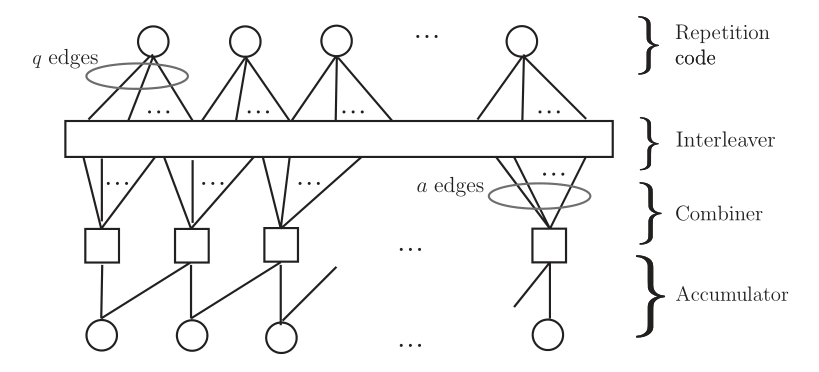
\includegraphics[width=0.85\linewidth]{figures/Ra_tanner.png}}
\caption{Γράφημα \en{Tanner RA} κώδικα}
\label{fig:RA tanner graph}
\end{figure}

Στην περίπτωση που οι κόμβοι \en{parity bits} και συστηματικών \en{bits} αντιμετωπίζονται ως ενιαίοι κόμβοι \en{bits} ο αλγόριθμος \en{SPA} για \en{RA} κώδικα, ταυτίζεται με αυτόν για ένα \en{LDPC} που έχει τον ίδιο πίνακα $\mathbf{H}$. Σε αντίθετη περίπτωση απαιτούνται τροποποιήσεις για τη συμπλήρωση μιας επανάληψης του αλγορίθμου.

Τέλος, ως σύγκριση μεταξύ του \en{Sum-Product} αποκωδικοποιητή και της \en{turbo} αποκωδικοποίησης, αναφέρεται πως, ενώ στον \en{SPA} οι \en{parity bit} κόμβοι αποκωδικοποιούνται όμοια με τους \en{systematic bit} κόμβους, ο \en{turbo} αποκωδικοποιητής χρησιμοποιεί \en{BCJR} αποκωδικοποιητή με διάγραμμα \en{trellis}. Μέσω αυτού οι επαναλήψεις της \en{turbo} αποκωδικοποίησης είναι πιο πολύπλοκες, ωστόσο απαιτούνται λιγότερες επαναλήψεις συνολικά \cite{ryan2009channel}, \cite{johnson2009iterative}.
	\chapter{\selectlanguage{greek}Προσομοίωση \en{DVB-S2 RA} κώδικα σε κανάλι \en{AWGN}}
\externaldocument{chapter3.tex}
Στο κεφάλαιο αυτό, θα παρουσιαστεί ο δέκτης που προσομοιώθηκε και τα αποτελέσματα της προσομοίωσης σε καμπύλες \en{BER} για τους διάφορους ρυθμούς που έχουν προτυποποιηθεί για την ψηφιακή τηλεόραση δεύτερης γενιάς (\en{DVB-S/T2}).

Αρχικά παρουσιάζεται συνοπτικά η διαμόρφωση \en{QPSK} και κατόπιν η διαδικασία αποδιαμόρφωσης (\en{demapping}), μέσω ων έτοιμων συναρτήσεων που παρέχονται από το \en{MATLAB}, καθώς και μέσω ενός \en{A-Posteriori Probability (APP) demapper} που προγραμματίστηκε για το σκοπό αυτό. Στη συνέχεια παρουσιάζεται το σύνολο της προσομοίωσης και στο τέλος του κεφαλαίου, τα αποτελέσματά της.

\section{\en{QPSK Demapper}}
\subsection{Διαμόρφωση \en{QPSK}}
Η κωδική λέξη, μετά την έξοδό της από τον κωδικοποιητή καναλιού, απεικονίζεται στον \en{QPSK} αστερισμό και προκύπτει η ακολουθία μιγαδικών σημάτων, μήκους $n/2$. Σε μορφή ημιτονοειδών κυμάτων μετάδοσης, ο \en{QPSK} αστερισμός γράφεται ως εξής:

\begin{equation}
s_n(t)=\sqrt{\frac{2E_s}{T_s}}\cos\left(2{\pi}f_ct+(2m-1)\frac{\pi}{4}\right),\;\;\;m=1,2,3,4.
\label{eq:QPSK sinusoid waves}
\end{equation}
όπου $E_s$ η ενέργεια συμβόλου, $T_s$ η διάρκεια συμβόλου, $f_c$ η συχνότητα του φέροντος κύματος και $m$ ο δείκτης των συμβώλων. Το αποτέλεσμα είναι ένας δι-διάστατος χώρος σημάτων με μοναδιαίες συναρτήσεις βάσης:

\begin{equation}
\begin{aligned}
\phi_1=\sqrt{\frac{2}{T_s}}\cos(2{\pi}f_ct) \\ \phi_2=\sqrt{\frac{2}{T_s}}\sin(2{\pi}f_ct)
\end{aligned}
\label{eq:QPSK base functions}
\end{equation}
όπου $\phi_1$ είναι η συμφασική και $\phi_2$ η ορθογώνια συνιστώσα. Το σήμα αποτυπώνεται στα 4 σημεία του αστερισμού \en{QPSK} $\left(\pm\sqrt{E_s/2},\pm\sqrt{E_s/2}\right)$ και οι φάσεις των συμβώλων προκύπτουν $\pi/4$, $3\pi/4$, $5\pi/4$ και $7\pi/4$. Ο παραπάνω αστερισμός φαίνεται στο Σχήμα \ref{fig:qpsk constellation}:

\begin{figure}[h]
\center{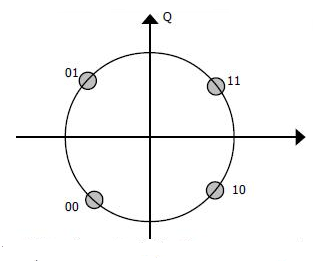
\includegraphics[width=0.55\linewidth]{figures/qpsk_constellation_diagram.png}}
\caption{Ο αστερισμός \en{QPSK}}
\label{fig:qpsk constellation}
\end{figure}
\hfill\\

Στη συνέχεια το σήμα περνάει από το κανάλι μετάδοσης, όπου προστίθεται το \en{AWGN} θόρυβος. Στο δέκτη ακολουθείται η αντίστροφη διαδικασία. Το \en{Matlab} παρέχει έτοιμη μέθοδο αποδιαμόρφωσης και ανίχνευσης μέσω του αντικειμένου \en{comm.QPSKDemodulator} και της μεθόδου \en{step}.

Για την προσομοίωση, προγραμματίστηκε επίσης και ο εξής \en{APP symbol-to-bit demapper}: μετά την έξοδο από το κανάλι η ακολουθία μιγαδικών αριθμών $\mathbf{y}$ μήκους $n/2$ εισάγεται στον \en{demapper}, ο οποίος παράγει μετρικές $L(x_{ij})$ στο διάστημα $(-\infty,\infty)$ για καθένα από τα κωδικά \en{bits} $x_{ij}$, σύμφωνα με τη σχέση:

\begin{equation}
L(x_{ij})=\ln\frac{p(x_{ij}=0\mid\mathbf{y}_i)}{p(x_{ij}=1\mid\mathbf{y}_i)},\;\;\;i\in\left[1,\frac{n}{2}\right],j=1,2.
\label{eq:QPSK LLR}
\end{equation}
οι οποίες εισάγονται στον επαναληπτικό αποκωδικοποιητή για την αρχικοποίησή του.

Από τις εξισώσεις \ref{eq:QPSK sinusoid waves}, \ref{eq:QPSK base functions} προκύπτει πως η διαμόρφωση \en{QPSK} αποτελεί απεικόνιση των δυάδων $\{0,1\}^2$, οι οποίες καλούνται \textit{ετικέτες} (\en{labels}), στο σύνολο των \en{QPSK} σημάτων $S$, δηλαδή $\{0,1\}^2\to{S}$. Αν συμβολιστέι ως ${S}_0^j$  το υποσύνολο των στοιχείων του $S$ που στην \en{j}-οστή θέση της ετικέτας του έχουν 0 και ως ${S}_1^j$ το υποσύνολο των στοιχείων του $S$ που στην \en{j}-οστή θέση της ετικέτας του έχουν 1 και θεωρηθεί απεικόνιση \en{Gray}, προκύπτουν σχηματικά τα υποσύνολα του Σχήματος \ref{fig:qpsk subtotals}.

\begin{figure}[h]
\center{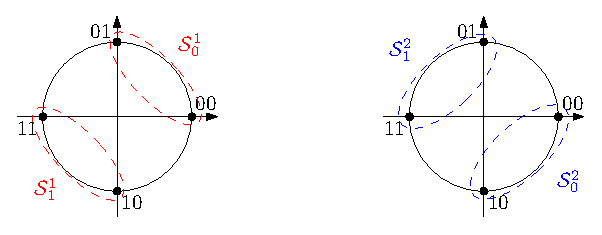
\includegraphics[width=0.55\linewidth]{figures/qpsk.eps}}
\caption{Τα υποσύνολα $ \color{red} {S}_1^0$, $ \color{red} {S}_1^1$ και $ \color{blue} {S}_0^0$, $ \color{blue}{S}_0^1$}
\label{fig:qpsk subtotals}
\end{figure}

Η σχέση \ref{eq:QPSK LLR} μπορεί να αναλυθεί περεταίρω για το κωδικό \en{bit} $L(x_{i1})$, αν εφαρμοστεί ο νόμος ολικής πιθανότητας, επιμερίζοντας σε όλα τα γεγονότα $x_{i2}$, το γεγονός $\{x_{i1}=0\}$ στον αριθμητή και το $\{x_{i1}=1\}$ στον παρονομαστή, ώστε να πάρει την μορφή της εξίσωσης \ref{eq:fraction 4.1}:

\begin{equation}
\begin{split}
L(x_{i1}) & =\ln\frac{\sum\nolimits_{x_{i2}}p(x_{i1}=0, x_{i2}\mid\mathbf{y}_i)}{\sum\nolimits_{x_{i2}}p(x_{i1}=1, x_{i2}\mid\mathbf{y}_i)} \\
& = \ln\frac{\sum\nolimits_{\mathbf{s}\in{S}_0^1} p(\mathbf{s}\mid\mathbf{y}_i)}{\sum\nolimits_{\mathbf{s}\in{S}_1^1} p(\mathbf{s}\mid\mathbf{y}_i)}
\end{split}
\label{eq:fraction 4.1}
\end{equation}

Γενικεύοντας από την εξίσωση \ref{eq:fraction 4.1}, για το κωδικό \en{bit} $L(x_{ij})$, προκύπτει:

\begin{equation}
\begin{split}
L(x_{ij}) & = \ln\frac{\sum\nolimits_{\mathbf{s}\in{S}_0^j} p(\mathbf{s}\mid\mathbf{y}_i)}{\sum\nolimits_{\mathbf{s}\in{S}_1^j} p(\mathbf{s}\mid\mathbf{y}_i)} \\
& = \ln\frac{\sum\nolimits_{\mathbf{s}\in{S}_0^j} p(\mathbf{y}_i\mid\mathbf{s})p(\mathbf{s})}{\sum\nolimits_{\mathbf{s}\in{S}_1^j} p(\mathbf{y}_i\mid\mathbf{s})p(\mathbf{s})} \\
& = \ln\frac{\sum\nolimits_{\mathbf{s}\in{S}_0^j} p(\mathbf{y}_i\mid\mathbf{s})}{\sum\nolimits_{\mathbf{s}\in{S}_1^j} p(\mathbf{y}_i\mid\mathbf{s})}
\end{split}
\label{eq:fraction 4.2}
\end{equation}

Οι ισότητες λογαρίθμων στην εξίσωση \ref{eq:fraction 4.2} προκύπτουν χρησιμοποιώντας τον κανόνα του \en{Bayes} και υποθέτοντας ότι τα σήματα $\mathbf{s} \in S$ είναι ισοπίθανα.

Ακόμη για το διακριτό κανάλι \en{AWGN}, η κατανομή πυκνότητας πιθανόητας $p(\mathbf{y}_i\mid\mathbf{s})$ ορίζεται ως εξής:

\begin{equation}
p(\mathbf{y}_i\mid\mathbf{s})=\frac{1}{2\pi\sigma^2}\exp\left\{-\frac{{\norm{\mathbf{y}_i-\mathbf{s}}}^{2}}{2\sigma^2}\right\}
\label{eq:AWGN pdf}
\end{equation}

Συνοψίζοντας, η εξίσωση \ref{eq:fraction 4.1}, λόγω των \ref{eq:fraction 4.2}, \ref{eq:AWGN pdf} γίνεται:

\begin{equation}
\begin{split}
L(x_{ij}) & =\ln \frac{\sum \nolimits_{\mathbf{s}\in{S}_0^j} \exp \left\{ -\frac{\norm{\mathbf{y}_i}^2 -2\Re(\mathbf{y}_i\cdot\mathbf{s}) + \norm{\mathbf{s}}^2}{2\sigma^2} \right\}}{\sum \nolimits_{\mathbf{s}\in{S}_1^j} \exp \left\{ -\frac{\norm{\mathbf{y}_i}^2 -2\Re(\mathbf{y}_i\cdot\mathbf{s}) + \norm{\mathbf{s}}^2}{2\sigma^2} \right\}} \\
& =\ln \frac{\sum \nolimits_{\mathbf{s}\in{S}_0^j} \exp \left\{ \frac{\Re(\mathbf{y}_i\cdot\mathbf{s})}{\sigma^2}\right\}}{\sum \nolimits_{\mathbf{s}\in{S}_1^j} \exp \left\{ \frac{\Re(\mathbf{y}_i\cdot\mathbf{s})}{\sigma^2}\right\}}
\end{split}
\label{eq:fraction 4.3}
\end{equation}

Στην εξίσωση \ref{eq:fraction 4.3}, θεωρώντας πως η ενέργεια σήματος $\norm{\mathbf{s}}^2=E_s,\;\forall \; \mathbf{s} \in S$ είναι η ίδια, οι παράγοντες $\exp\left\{-\frac{\norm{\mathbf{y}_i}^2}{2\sigma^2}\right\}$, $\exp\left\{-\frac{\norm{\mathbf{s}}^2}{2\sigma^2}\right\}$ μπορούν να απαλειφθούν με παραγοντοποίηση σε αριθμητή και παρονομαστή και τελικά η εξίσωση \ref{eq:fraction 4.3} να λάβει τη μορφή:

\begin{equation}
L(x_{ij})=\ln\frac{\sum \nolimits_{\mathbf{s}\in{S}_0^j}\exp\left\{\frac{y_{iI}s_I+y_{iQ}s_Q}{\sigma^2}\right\}}{\sum \nolimits_{\mathbf{s}\in{S}_1^j}\exp\left\{\frac{y_{iI}s_I+y_{iQ}s_Q}{\sigma^2}\right\}}
\label{eq:fraction 4.4}
\end{equation}
όπου οι δείκτες $I$, $Q$ υποδεικνύουν προβολή του αντίστοιχου διανύσματος στη συμφασική και στην ορθογώνια συνιστώσα αντίστοιχα.

\section{Προσομοίωση στο \en{Matlab}}
% \selectlanguage{english}
% {spa9.m}
% 
\begin{table}[h]
\centering
\begin{tabular}
{>{\bfseries}c*{2}{c}}\toprule\toprule{\en{Rate R}} & {$(E_b/N_0)_{soft}\;\;(dB)$}\\ \midrule
1/4&-0.793\\
1/3&-0.497\\
2/5&-0.236\\
1/2&0.187\\
3/5&0.682\\
2/3&1.059\\
3/4&1.626\\
4/5&2.039\\
9/10&3.199\\ \bottomrule\bottomrule
\end{tabular}
\caption{Χωρητικότητα ως \en{$E_b/N_0$} για τους ρυθμούς κώδικα της προσομοίωσης}
\label{table: EbN0 limits}
\end{table}

Στον πίνακα \ref{table: EbN0 limits}, φαίνεται το (θεωρητικό) κάτω όριο $E_b/N_0$ για τον κάθε ρυθμό κώδικα που προσομοιώνεται, το οποίο καλείται \textit{όριο κωδικοποίησης} και αντιστοιχεί σε διαμόρφωση \en{BPSK} ή \en{QPSK}. Η χωρητικότητα, όπως εκφράζεται από τα παραπάνω όρια για δεδομένο ρυθμό \en{R}, δίνει ένα κατώφλι \en{SNR} μετά από το οποίο και με τη χρήση κωδικοποίησης καναλιού, μπορεί να επιτευχθεί -θεωρητικά- αξιόπιστη επικοινωνία, σε διαφορετική περίπτωση η αξιοπιστία της οποίας είναι μη ελέγξιμη.

Για να υλοποιηθεί προσομοίωση στο \en{Matlab} μεταβάλλεται η μεταβλητή \en{R} η οποία αποθηκεύει το ρυθμό του κώδικα και ορίζεται ο \en{LDPC} κώδικας με βάση τον πίνακα $\mathbf{H}$. Κατόπιν αρχικοποιούνται τα αντικείμενα που ορίζουν τις παραμέτρους της διαμόρφωσης-αποδιαμόρφωσης και κωδικοποίησης-αποκωδικοποίησης. Ωστόσο, η συνάρτηση \en{demod} δε χρησιμοποιείται, καθώς για τη συγκεκριμένη προσομοίωση γίνεται χρήση του \en{APP demapper} που περιγράφηκε στην προηγούμενη παράγραφο του κεφαλαίου.

\tl{\lstinputlisting{def.m}}
\tl{\lstinputlisting{encdec.m}}
\tl{\lstinputlisting{moddemod.m}}

Η κωδικοποίηση γίνεται σύμφωνα με όσα αναφέρθηκαν στο Κεφάλαιο 3 και ακολουθεί την συστηματική \en{LDPC}, σύμφωνα με το πρότυπο \en{Digital Video Broadcasting \& Satellite - Second Generation (DVB-S2)} \cite{etsi2009302}. Όπως φαίνεται από το παραπάνω κομμάτι κώδικα, το αντικείμενο \textit{\en{enc}} αρχικοποιείται με βάσει τον πίνακα ελέγου ισοτιμίας για δεδομένο ρυθμό κώδικα. Διακρίνεται από τα εξής βήαματα:

\begin{itemize}
\item Αρχικοποίηση των \en{parity bits}: $p_0=p_1=\cdots=p_{n-k-1}=0$
\item Συσσώρευση του πρώτου \en{info bit} στις διευθύνσεις που δίνονται από την πρώτη γραμμή των πινάκων \en{B.1} έως \en{B.11} του παραρτήματος Β στο πρότυπο \en{ETSI} για το \en{DVB-S2} \cite{etsi2009302}, με \en{mod}-2 πρόσθεση.
\item Για τα επόμενα 359 \en{info bits} οι διευθύνσεις των συσσωρευτών δίνονται από τον τύπο $\lbrace x+\left(m\; mod\; 360\right) \times q\rbrace mod \left(n-k\right)$, όπου $m=1,2,\cdots,359$, το $x$ αντιστοιχεί στη διεύθυνση συσσωρρευτή του πρώτου \en{info bit} και το $q$ δίνεται από τον Πίνακα \ref{table:q values}
\item Αντίστοιχα, για κάθε επόμενο \en{group} από 360 \en{info bits} χρησιμοποιείται μια καινούργια γραμμή διευθύνσεων στους πίνακες \en{B.1} έως \en{B.11} του παραρτήματος Β του \cite{etsi2009302}
\item Με την εξάντληση των \en{info bits}, τα τελικά \en{parity bits} $p_i$ δίνονται ως εξής:
\begin{equation*}
p_0 = p_0
\end{equation*}
\begin{equation*}
p_i = p_i \oplus p_{i-1},\;\;i=1,2,\cdots,n-k
\end{equation*}
\end{itemize}

\begin{table}[H]
\centering
\begin{tabular}
{>{\bfseries}c*{2}{c}}\toprule\toprule{\en{Code Rate}} & {$q$}\\ \midrule
1/4&135\\
1/3&120\\
2/5&108\\
1/2&90\\
3/5&72\\
2/3&60\\
3/4&45\\
4/5&36\\
9/10&18\\ \bottomrule\bottomrule
\end{tabular}
\caption{Τιμές $q$ για τους διάφορους ρυθμούς κωδικοποίησης \en{RA}}
\label{table:q values}
\end{table}

Αντίστοιχα η αποκωδικοποίηση στηρίζεται στην εφαρμογή του \en{SPA} αλγορίθμου για \en{LDPC} και ακολουθεί την παρακάτω πορεία:

\begin{itemize}
\item Η αρχικοποίηση των $L_j$ γινεται μέσω της σχέσης \ref{eq:AWGN initial LLR}
\item Τα μηνύματα που εξέρχονται απο τους \en{CN} υπολογίζονται από την εξίσωση 
\begin{equation}
L_{i\to j} = 2\tanh^{-1} \left( \prod_{j'\in N(i)-\lbrace j\rbrace} \tanh \left( \frac{1}{2}L_{j'\to i} \right)\right)
\end{equation}
και κατόπιν μεταδίδονται στους \en{VN}
\item Τα μηνύματα που εξέρχονται απο τους \en{VN} υπολογίζονται από την εξίσωση
\begin{equation*}
L_{j\to i} = L_j + \sum_{i'\in N(j)-\lbrace i\rbrace} L_{i'\to j}
\end{equation*}
και κατόπιν μεταδίδονται στους \en{CN}
\item Τα συνολικα \en{LLR} υπολογίζονται από τη σχέση
\begin{equation*}
L_{j}^{total} = L_j + \sum_{i\in N(j)} L_{i\to j}
\end{equation*}
\item Για $j=0,1,\cdots,n-1$ υπολογίζονται οι τιμές των \en{bit}
\begin{equation*}
\hat{v_j}=\left\{
\begin{array}{c l}	
     1 & L_{j}^{total}<0\\
     0 & else
\end{array}\right.
\end{equation*}
που διαμορφώνουν την $\hat{\mathbf{v}}$. Αν $\hat{\mathbf{v}}\mathbf{Η}=\mathbf{0}$, ο αλγόριθμος τερματίζει, αλλιώς συνεχίζει με την επόμενη επανάληψη.
\item Στο τέλος της προσομοίωσης υπολογίζονται οι μετρικές \en{BER} και \en{FER} για την προσομοίωση του εκάστοτε ρυθμού στο αντίστοιχο \en{SNR}
\end{itemize}


Η προσομοίωση έχει ως όριο τα $10^3$ σφάλματα ή τις $10^6$ προσπάθειες (\en{trials}) να εντοπιστούν. Τα αποτελέσματα που θα παρουσιαστούν, λαμβάνονται αφού αποθηκευτούν για κάθε ρυθμό το \en{Bit Error Rate - BER} και το \en{Frame Error Rate - FER}. Επίσης αποθηκεύεται ο απόλυτος αριθμός σφαλμάτων και ο αριθμός \en{trials} που χρειάστηκαν, για το συγκεκριμένο \en{SNR}.

\section{Αποτελέσματα}

Σε αυτό το σημείο παρουσιάζονται τα αποτελέσματα της προσομοίωσης. Τα διαγράμματα που ακολουθούν απεικονίζουν για κάθε ρυθμό του Πίνακα \ref{table: EbN0 limits} τις τιμές του \en{BER}, ξεκινώντας από την τιμή $Eb/N0$ του Πίνακα \ref{table: EbN0 limits} (θεωρητικό όριο χωρητικότητας για κάθε ρυθμό) και καταλήγοντας στη τιμή $Eb/N0$, για την οποία το \en{BER} φτάνει στο $10^{-8}$. Στό ίδιο διάγραμμα απεικονίζεται και η καμπύλη του \en{FER} για τις αντίστοιχες τιμές $Eb/N0$. Στο τέλος, δίνεται επίσης ένα συγκριτικό διάγραμμα όλων των καμπυλών \en{BER} και \en{FER}, για καλύτερη εποπτεία των αποτελεσμάτων των διαφόρων ρυθμών.
\begin{figure}[h]
\center{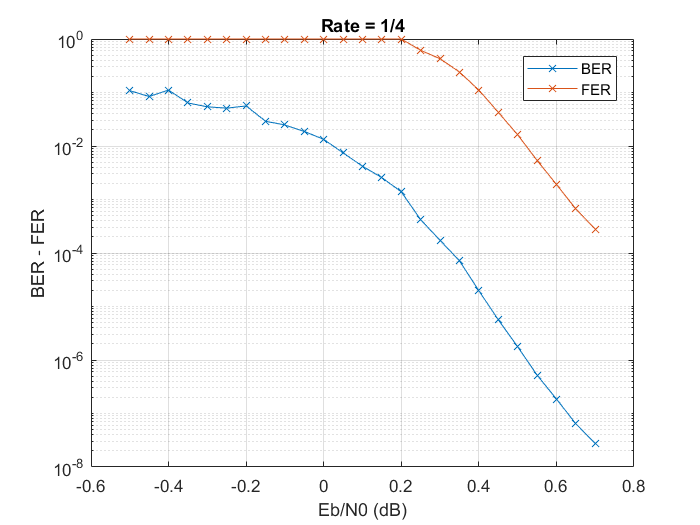
\includegraphics[width=0.75\linewidth]{matlab/1-4.png}}
\caption{\en{BER},\en{FER vs} $Eb/N0$ για ρυθμό 1/4}
\end{figure}
\begin{figure}[h]
\center{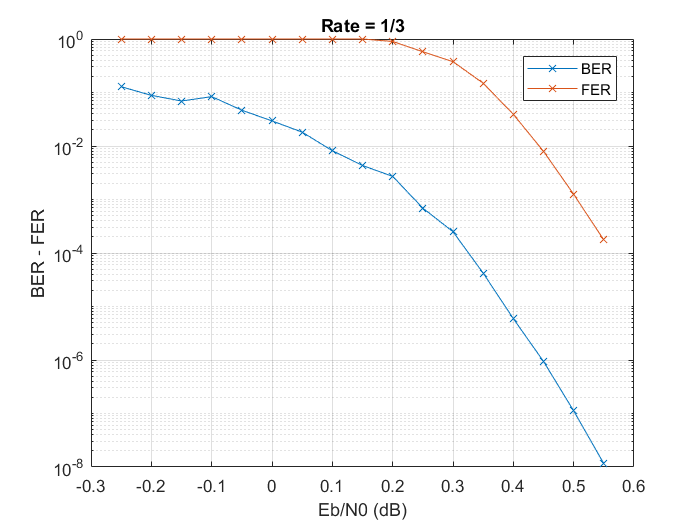
\includegraphics[width=0.75\linewidth]{matlab/1-3.png}}
\caption{\en{BER},\en{FER vs} $Eb/N0$ για ρυθμό 1/3}
\end{figure}
\begin{figure}[h]
\center{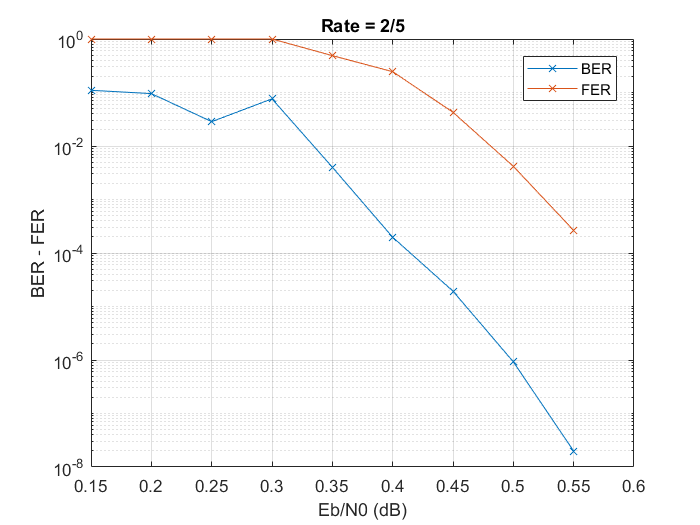
\includegraphics[width=0.75\linewidth]{matlab/2-5.png}}
\caption{\en{BER},\en{FER vs} $Eb/N0$ για ρυθμό 2/5}
\end{figure}
\begin{figure}[h]
\center{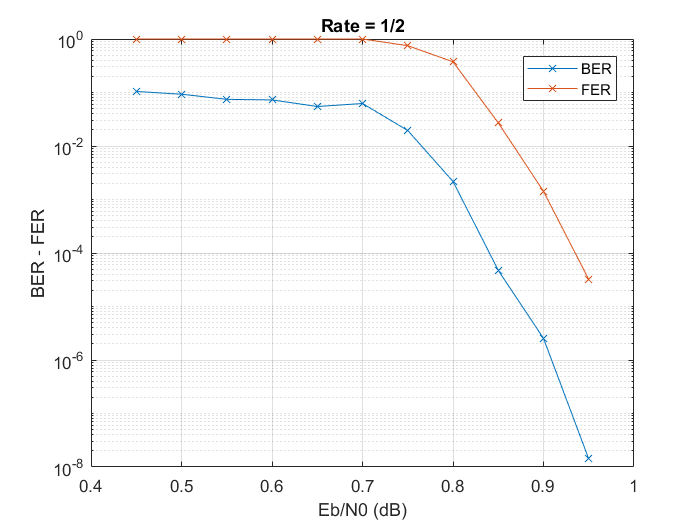
\includegraphics[width=0.75\linewidth]{matlab/1-2.png}}
\caption{\en{BER},\en{FER vs} $Eb/N0$ για ρυθμό 1/2}
\end{figure}
\begin{figure}[h]
\center{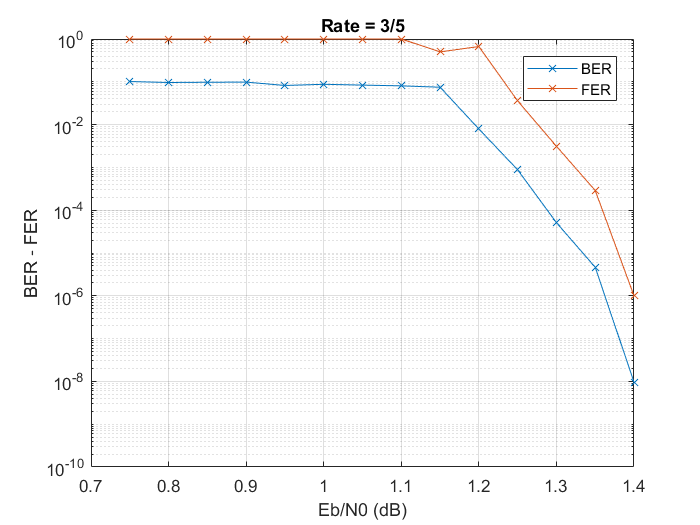
\includegraphics[width=0.75\linewidth]{matlab/3-5.png}}
\caption{\en{BER},\en{FER vs} $Eb/N0$ για ρυθμό 3/5}
\end{figure}
\begin{figure}[h]
\center{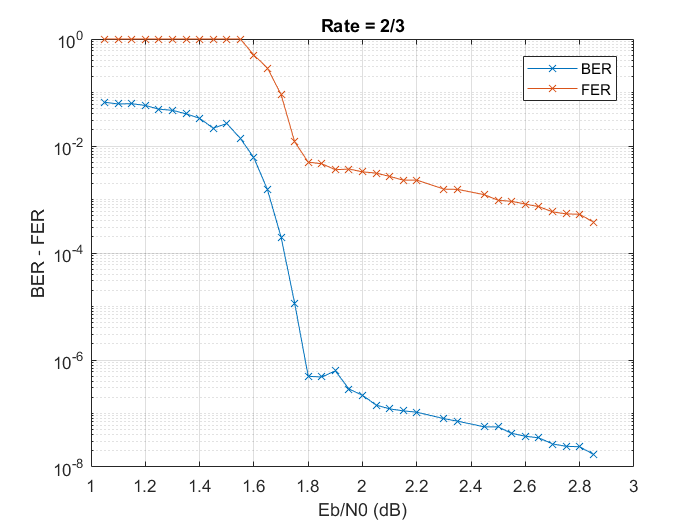
\includegraphics[width=0.75\linewidth]{matlab/2-3.png}}
\caption{\en{BER},\en{FER vs} $Eb/N0$ για ρυθμό 2/3}
\end{figure}
\begin{figure}[h]
\center{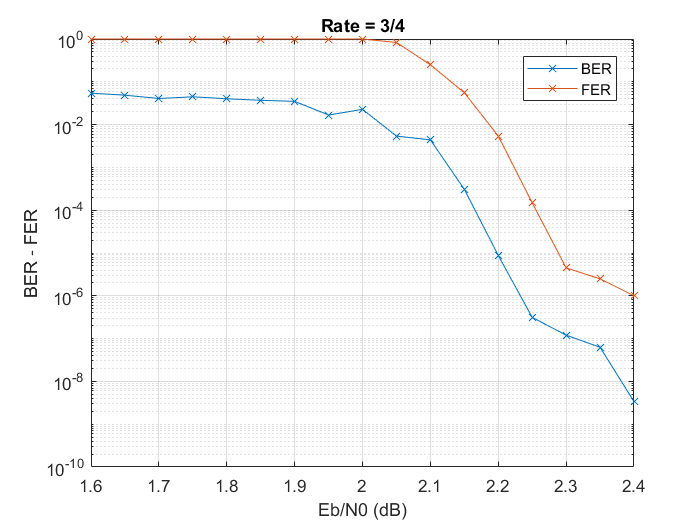
\includegraphics[width=0.75\linewidth]{matlab/3-4.png}}
\caption{\en{BER},\en{FER vs} $Eb/N0$ για ρυθμό 3/4}
\end{figure}
\begin{figure}[h]
\center{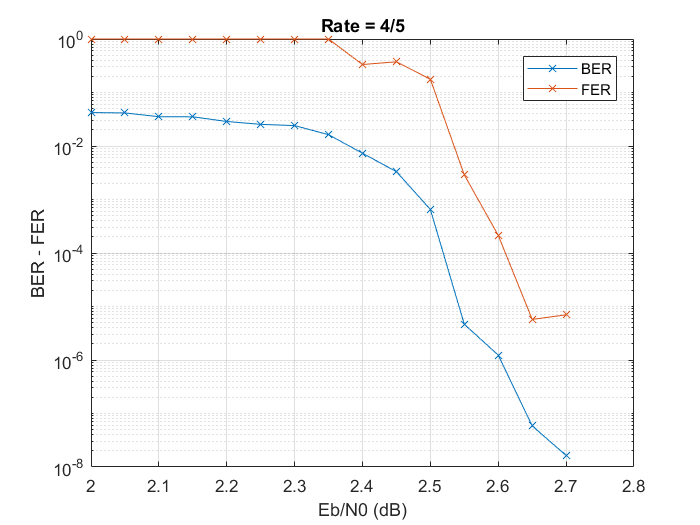
\includegraphics[width=0.75\linewidth]{matlab/4-5.png}}
\caption{\en{BER},\en{FER vs} $Eb/N0$ για ρυθμό 4/5}
\end{figure}
\begin{figure}[h]
\center{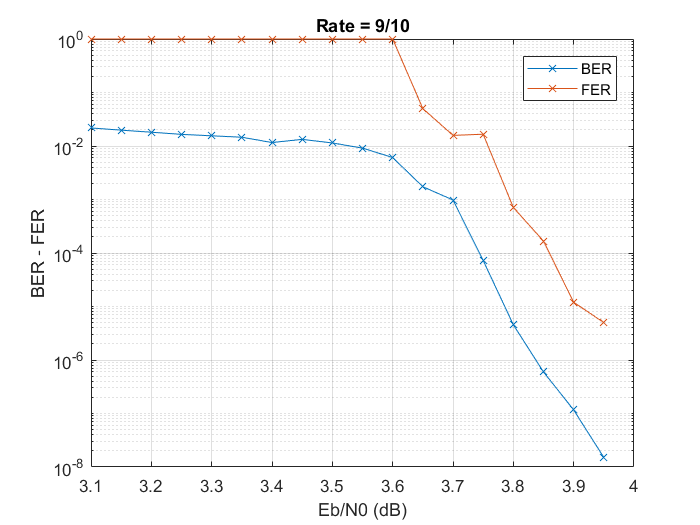
\includegraphics[width=0.75\linewidth]{matlab/9-10.png}}
\caption{\en{BER},\en{FER vs} $Eb/N0$ για ρυθμό 9/10}
\end{figure}

\begin{figure}[h]
\center{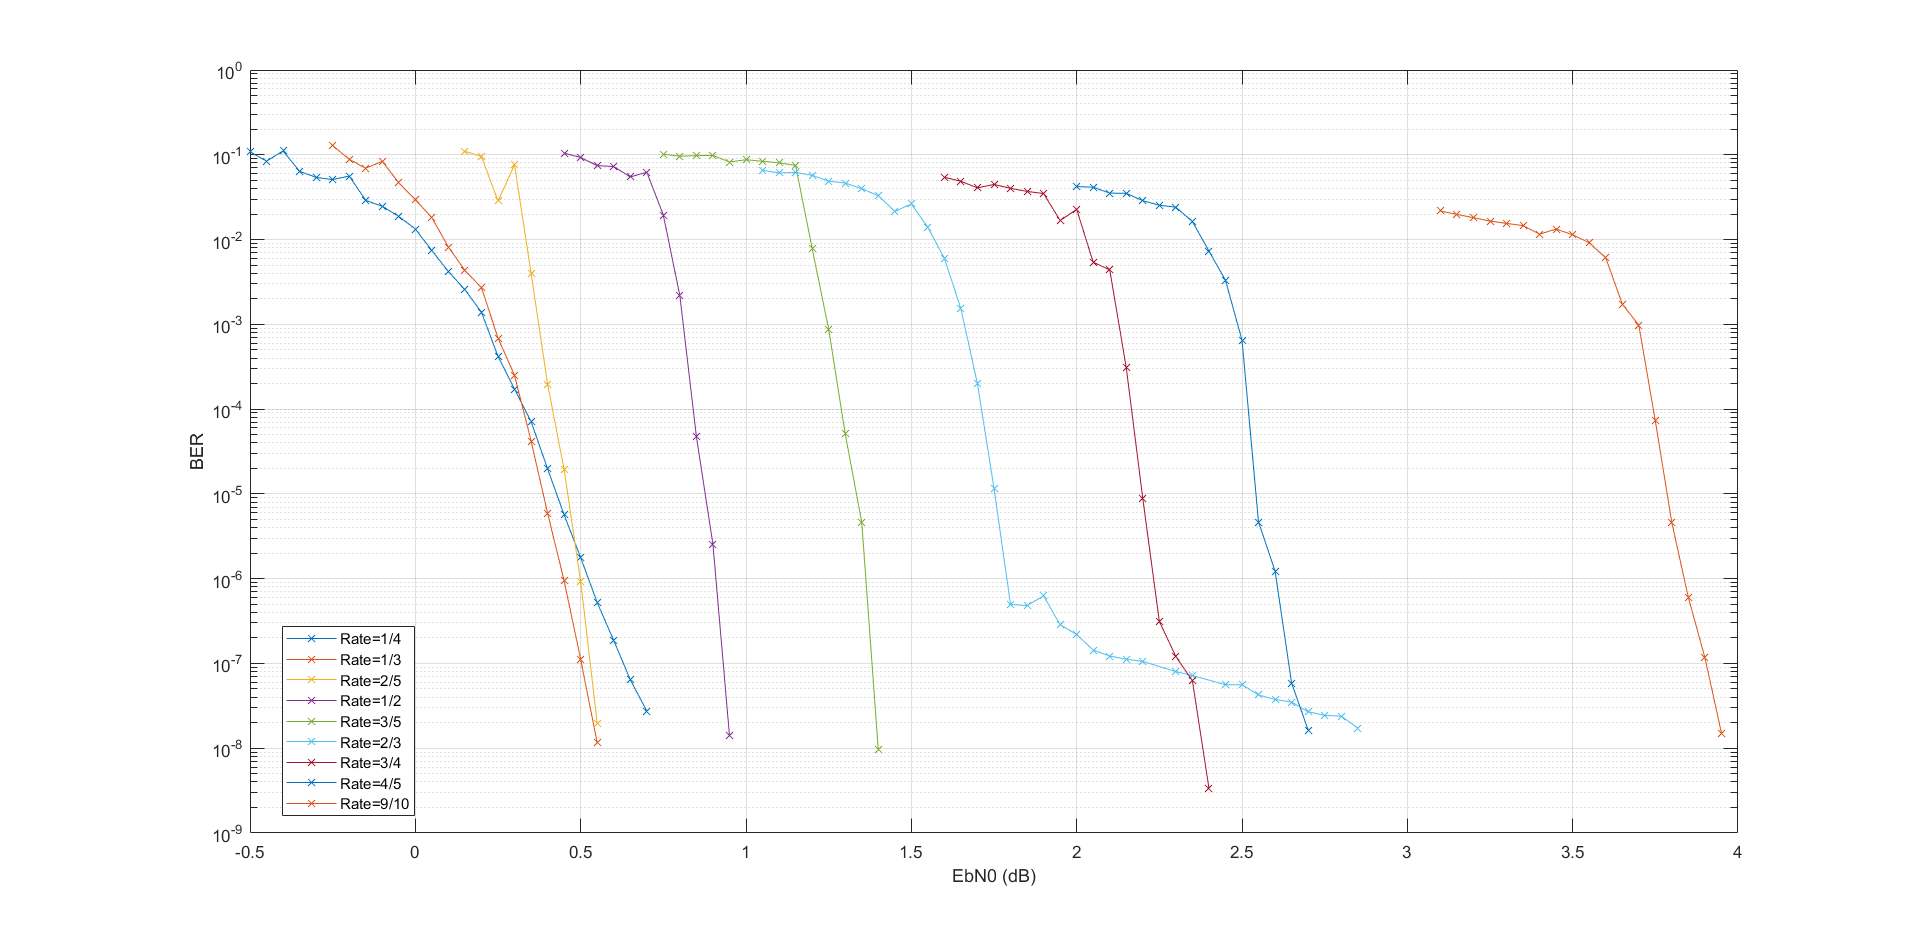
\includegraphics[width=1.0\linewidth]{matlab/full_BER.png}}
\caption{Καμπύλες \en{BER vs} $Eb/N0$ για διαφορετικούς ρυθμούς}
\end{figure}

\begin{figure}[h]
\center{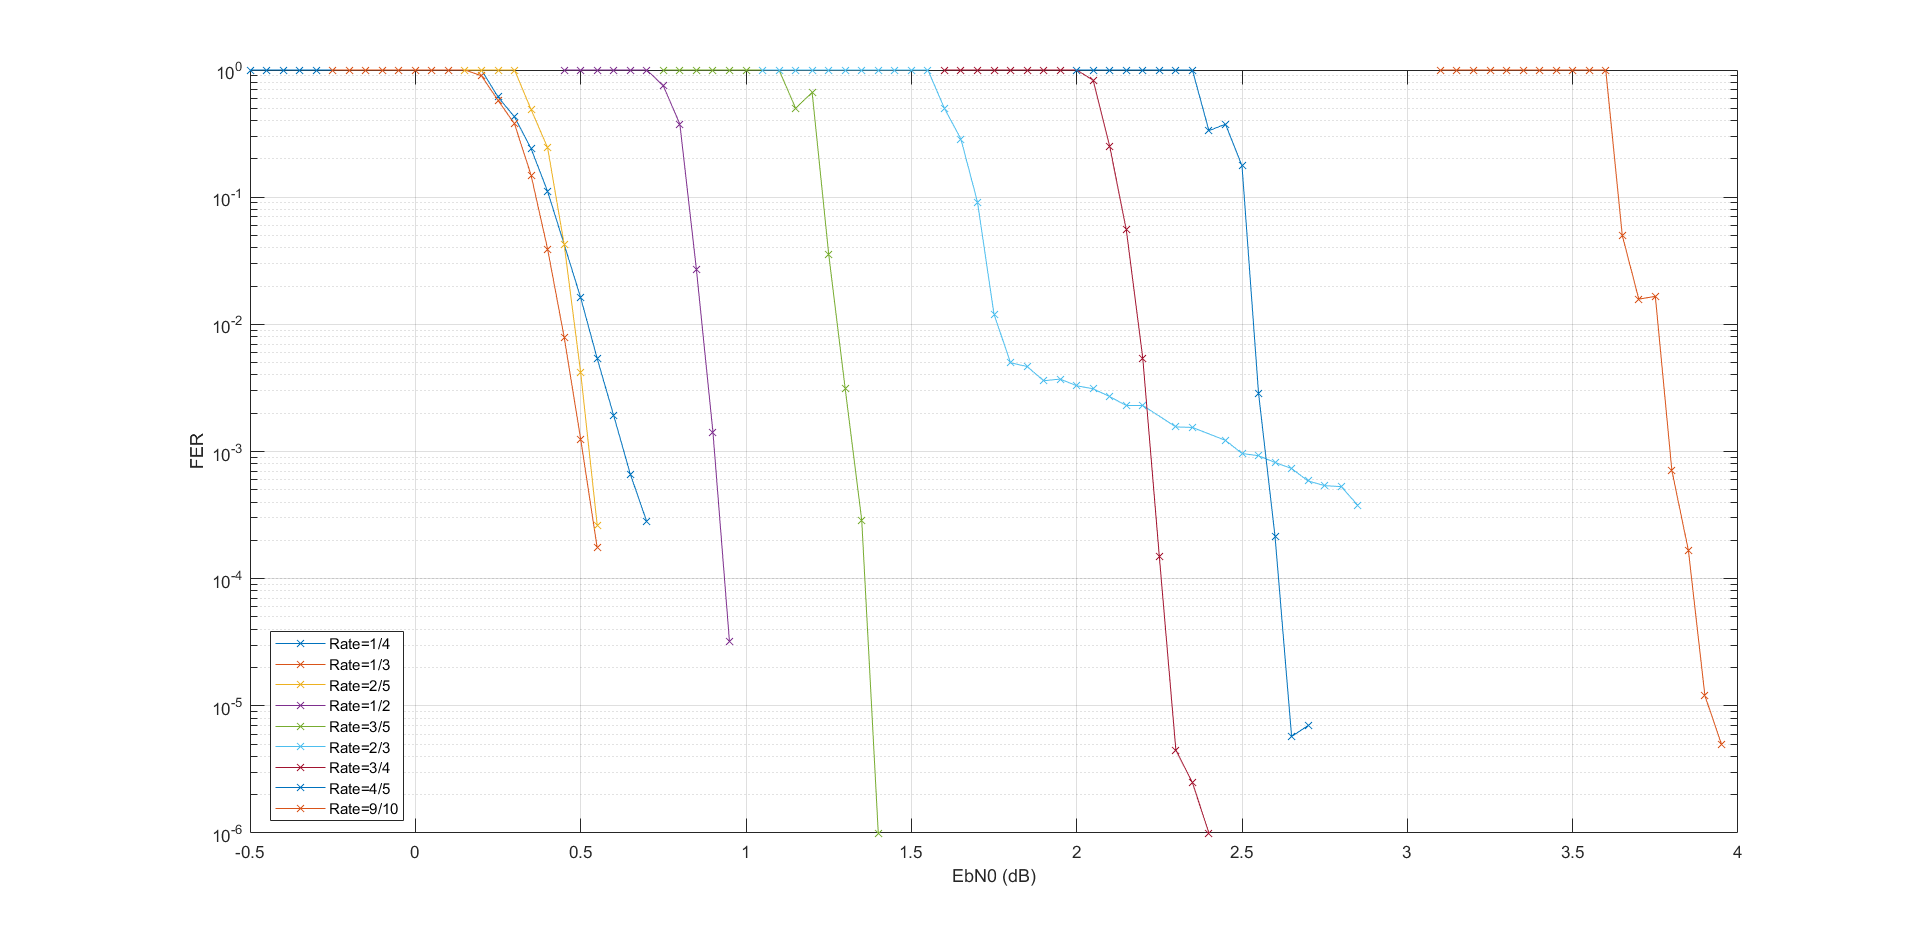
\includegraphics[width=1.0\linewidth]{matlab/full_FER.png}}
\caption{Καμπύλες \en{FER vs} $Eb/N0$ για διαφορετικούς ρυθμούς}
\end{figure}
	\chapter{\selectlanguage{greek}Mελλοντικές επεκτάσεις}
Στο Κεφάλαιο 3, αναφέρθηκε πως οι \en{VNs} είναι ανεξάρτητοι κόμβοι που μπορούν ο καθένας να υπολογίζει τα εξαγόμενα \en{LLR} παράλληλα με τους υπόλοιπους. Το ίδιο ισχύει και για τους \en{CNs}. Άρα ο αλγόριθμος \en{SPA} είναι από τη φύση τους έντονα παραλληλοποιήσιμος. Καθώς οι ασύρματες συσκευές μεταδίδουν και δέχονται δεδομένα υψηλού ρυθμού σε πραγματικό χρόνο, αυξάνεται ραγδαία η ανάγκη για ταχύτητα και αξιοπιστία στην επικοινωνία.

Η χρήση των \en{LDPC} σε πολλά νέα πρότυπα (\en{DVB-S2, WiMAX (802.16e), Wifi (802.11n), 10 Gbit Ethernet (802.3an), 5G}  κ.λ.π. \cite{falcao2011massively}, καθώς και σε πολλαπλούς ρυθμούς δεδομένων για τα διαφορετικά πρότυπα, έχουν κάνει ορατή τη δυσκολία για υλοποίηση \en{hardware}, καθώς η επεξεργασία βασικής ζώνης στο επίπεδο του φυσικού εξαρτήματος είναι πολυδάπανη σε εύρος ζώνης και επεξεργαστική ισχύ. 

Αντ\textquotesingle αυτού, ο σχεδιασμός συστημάτων ψηφιακής τηλεπικοινωνίας υιοθετεί όλο και περισσότερο υλοποιήσεις σε \en{software}, μέσω της χρήσης \en{CPUs} ή/και \en{GPU} \cite{park2011parallel}, \cite{abburi2011scalable}. Σχετική έρευνα, έχει δείξει τη διαφορά στη χρήση \en{GPU} σε σχέση με κυκλώματα \en{ASIC} για \en{LDPC} αποκωδικοποίηση \cite{falcao2009gpus}.

\section{Προσομοίωση σε \en{CUDA}}

Η χρήση προγραμματισμού σε \en{GPU} προσφέρει υψηλή υπολογιστική ισχύ, καθώς οι μονάδες επεξεργασίας γραφικών αποκτούν ολοένα και καλύτερες επιδόσεις. Προς την κατεύθυνση αυτή, αξιοσημείωτο ενδιαφέρον παρουσιάζει ο προγραμματισμός με βάση την αρχιτεκτονική \en{Compute Unified Device Architecture (CUDA)} της εταιρίας \en{nVidia}.

Σχετική έρευνα έχει υπάρξει αναφορικά με τη χρήση \en{GPU} για τη διαχείρηση του \en{SPA} και την εξαγωγή πληροφορίας από τις μετρικές \en{LLR} \cite{falcao2009parallel}. Ακόμη, υπάρχει προτεινόμενος τρόπος για την υλοποίηση \en{CUDA} για χρήση \en{LDPC} αποκωδικοποίησης \cite{falcao2011massively}, καθώς και υβριδική συνδυαστική χρήση \en{multicore CPU - GPU}, για την ενσωμάτωση πολλαπλών ρυθμών και τηλεπικοινωνιακών προτύπων \cite{park2011parallel}.

Με βάση, λοιπόν, τα παραπάνω αποκτά ενδιαφέρον η μελέτη προς την κατεύθυνση της ταχύτερης υλοποίησης \en{RA} αποκωδικοποιητών κάνοντας χρήση της αρχιτεκτονικής \en{CUDA}, καθώς και η μέτρηση και παρουσίαση των επιδόσεων τους.

% Παραρτήματα
	\appendix
	\chapter{Παράδειγμα Παραρτήματος}

% \section{Πρώτη ενότητα}
% Τα συστήματα ομότιμων κόμβων, προκειμένου να υποστηρίζουν πιο
% εκφραστικές λειτουργίες αναπαράστασης και αναζήτησης δεδομένων,
% εξελίχθηκαν στα συστήματα ομότιμων κόμβων τα οποία βασίζονται στις
% τεχνολογίες του Σημασιολογικού Ιστού για την αναπαράσταση των
% δεδομένων μέσω σχημάτων που τα περιγράφουν (\en{Schema-based
% peer-to-peer systems}).

% Συμπερασματικά το σύστημα που αναπτύχθηκε στα πλαίσια αυτής της
% διπλωματικής είναι ένα πλήρες σύστημα ομότιμων κόμβων βασισμένο σε
% σχήματα, το οποίο καθιστά δυνατή την αναζήτηση της πληροφορίας με
% ένα διαφορετικό τρόπο απ' ότι τα προϋπάρχοντα  συστήματα.

% \section{Μελλοντικές Επεκτάσεις}
% Το σύστημα που αναπτύχθηκε στα πλαίσια αυτής της διπλωματικής
% εργασίας θα μπορούσε να βελτιωθεί και να επεκταθεί περαιτέρω,
% τουλάχιστον ως προς τρεις κατευθύνσεις. Συγκεκριμένα, αναφέρονται
% τα ακόλουθα:

% \begin{itemize}
% \item Ενσωμάτωση διαδικασίας επιλογής σχήματος με βάση το οποίο ο
% κόμβος θα συμμετέχει στο σύστημα. Έτσι όπως έχει σχεδιαστεί το
% σύστημα, κάθε κόμβος έχει τη δυνατότητα να δημιουργήσει πολλά
% σχήματα και να αποθηκεύσει δεδομένα σε περισσότερα από ένα. Ως
% σχήμα του κόμβου (με βάση το οποίο απαντάει τις ερωτήσεις),
% θεωρείται το τελευταίο στο οποίο αποθήκευσε δεδομένα. Η δυνατότητα
% επιλογής θα του παρείχε περισσότερη ευελιξία.
% \item Δυνατότητα αντιστοίχισης δεδομένων τα οποία να μην είναι
% αποθηκευμένα σε βάση δεδομένων αλλά σε αρχεία. Η αποδέσμευση από
% τη βάση δεδομένων θα έκανε το σύστημα πιο εύκολο στην εγκατάσταση
% και τη χρήση.
% \item Αξιολόγηση του συστήματος ως προς τη συμπεριφορά του αν
% συμμετέχει σε αυτό μεγάλος αριθμός κόμβων \en{(scalability
% testing)} και αν χρησιμοποιηθεί ένα πολύ μεγάλο καθολικό σχήμα. H
% αξιολόγηση αυτή αφορά την ταχύτητα με την οποία ένας κόμβος
% παίρνει απαντήσεις σε μια ερώτηση καθώς και την ποιότητα των
% απαντήσεων.
% \end{itemize}

% %
% 	\begin{table}[!tb]
% 		\centering
% 		\caption{Πίνακας αλήθειας της λογικής συνάρτησης \en{F}}
% 		\small
% 		\renewcommand{\arraystretch}{1.3}
% 		\begin{tabular}{| c | c | c || c |}
% 			\hline               
% 		  	\textbf{\en{A}} & \textbf{\en{B}} &  \textbf{\en{C}} &   \textbf{\en{F}} \\
% 			\hline
% 				  0 & 0 & 0 & 0  \\
% 				  0 & 0 & 1 & 0  \\
% 				  0 & 1 & 0 & 1  \\
% 				  0 & 1 & 1 & 0  \\	
% 				  1 & 0 & 0 & 1  \\
% 				  1 & 0 & 1 & 0  \\
% 				  1 & 1 & 0 & 1  \\
% 				  1 & 1 & 1 & 0  \\
% 		  	\hline
% 		\end{tabular}
% 		\label{tableAppA.01}
% 	\end{table}
% %
	\cleardoublepage
% Βιβλιογραφία - Αναφορές
	\bibliography{references}
% % Συντομογραφίες - Αρκτικόλεξα - Ακρωνύμια
% 	\newcommand{\abbrevEN}[2]{\en{#1} \> \en{#2}\\ }
\newcommand{\abbrevGR}[2]{#1 \> #2\\ }

\chapter*{Συντομογραφίες - Ακρωνύμια}

\begin{tabbing}
%ta 'a' rythmizoun to platos ton dyo stilon
  aaaaaaaaaaaaaaaaa \= aaaaaaaaaaaaaaaaaaaaaa\kill
  \abbrevGR{βλπ}{βλέπε}
  \abbrevGR{δηλ.}{δηλαδή}
  \abbrevGR{κ.λπ.}{και λοιπά}
  \abbrevGR{κ.ο.κ}{και ούτω καθεξής}
  \abbrevGR{ανν}{αν και μόνον αν}
  \abbrevEN{AWGN}{Additive White Gaussian Noise}
  \abbrevEN{QPSK}{Quadrature Phase-Shifting Keying}
  \abbrevEN{LDPC}{Low Density Parity Check}
  \abbrevEN{DVB-S2}{Digital Video Broadcasting - Satellite 2}
  \abbrevEN{BER}{Bit Error Rate}
  \abbrevEN{SNR}{Signal-to-Noise Ratio}
  
\end{tabbing}
% % Γλωσσάριο
% 	\newcommand{\gloss}[2]{#1 \> \en{#2}\\ }

\chapter*{Απόδοση ξενόγλωσσων όρων}

\begin{tabbing}
%ta 'a' rythmizoun to platos ton dyo stilon
  aaaaaaaaaaaaaaaaaaaaaaaaaaaaaaaaaaa \= aaaa\kill
  \Large\textbf{Απόδοση} \> \Large\textbf{Ξενόγλωσσος όρος} \\
  \gloss{αδερφός}{sibling}
  \gloss{αμεταβλητότητα}{idempotency}
  %\gloss{αναγνωριστής}{identifier}
  \gloss{ανάκτηση πληροφορίας}{information retrieval}
  \gloss{αντιμεταθετικότητα}{commutativity}
  \gloss{απόγονος}{descedant}
  \gloss{απορρόφηση}{absorption}
  \gloss{βάση δεδομένων}{database}
  \gloss{γνώρισμα}{attribute}
  \gloss{διαπροσωπεία}{interface}
  \gloss{διαφορά}{difference}
  \gloss{δικτυακός κατάλογος}{portal catalog}
  \gloss{δικτυωτή δομή}{lattice}
  \gloss{δομικές επερωτήσεις}{structural queries}
  \gloss{δομικές σχέσεις}{structural relationships}
  \gloss{δομικό σχήμα}{schema}
  \gloss{εγκυρότητα}{validity}
  \gloss{ένωση}{union}
\end{tabbing}
%%%%%%%%%%%%%%%%%%%%%%%%%%%%%%%%%%%%%%%%%%%%%%%%%%%%
% \backmatter
% % Ευρετήριο Όρων
% 	\printindex
% 	\cleardoublepage

%%%%%%%%%%%%%%%%%%
%%%%%%%%%%%%%%%%%%

% 	\thispagestyle{empty}
\end{document}
